%
\documentclass[12pt, oneside, reqno]{article}
\usepackage{amssymb, amsthm, amsmath,amscd, amsfonts}
\usepackage{graphics}
\usepackage[pdftex]{graphicx}
\usepackage{charter}
\usepackage{color}% http://ctan.org/pkg/color
\usepackage[linkbordercolor={1 0 1}]{hyperref}
\hypersetup{linktocpage}
\renewcommand{\ttdefault}{ptm}
\usepackage{mathpazo}
\pdfpagewidth 8.5in
\pdfpageheight 11in
\usepackage{listings}
\lstset{language=R}

%--- Page structure ---

%\addtolength{\hoffset}{-2cm}
%\addtolength{\textwidth}{4cm}
 \DeclareMathOperator{\Tr}{Tr}
\renewcommand{\baselinestretch}{1.1}
\setlength{\voffset}{-.7truein}
\setlength{\textheight}{8.8truein}
\setlength{\textwidth}{6.05truein}
\setlength{\hoffset}{-.7truein}

%--------------------Environments--------------------------
\theoremstyle{definition}
\newtheorem{acknowledgement}{Acknowledgement}
\newtheorem{axiom}{Axiom}
\newtheorem{comment}{Comment}
\newtheorem{theorem}{\textbf{\textsc{Theorem}}}
\newtheorem{proposition}{\textbf{\textsc{Proposition}}}
\newtheorem{lemma}{\textbf{\textsc{Lemma}}}
\newtheorem{corollary}{\textbf{\textsc{Corollary}}}
\newtheorem{remark}{\textbf{\textsc{Remark}}}
\newtheorem{case}{Case}
\newtheorem{conclusion}{Conclusion}
\newtheorem{condition}{Condition}
\newtheorem{criterion}{Criterion}
\newtheorem{notation}{Notation}
\newtheorem{problem}{Problem}
\newtheorem{solution}{Solution}
\newtheorem{summary}{Summary}
\newtheorem{exercise}{Execrise}
\newtheorem{example}{Example}
\renewcommand{\ttdefault}{ptm}
\newtheorem*{discussion}{Discussion}
\newtheorem{definition}{\textbf{\textsc{Definition}}}

%--------------------Environments--------------------------

%---------------------Style File---------------------------
\newcommand{\R}{\mathbb{R}}
\newcommand{\U}{\mathcal{U}}
\newcommand{\OX}{\overline{x}}
\newcommand{\C}{\mathbb{C}}
\newcommand{\X}{\mathbf{X}}
\newcommand{\x}{\mathbf{x}}
\newcommand{\Z}{\mathbb{Z}}
\newcommand{\Q}{\mathbb{Q}}
\newcommand{\N}{\mathbb{N}}
\newcommand{\RR}{\mathcal{R}}
\newcommand{\OP}{\overline{\partial}}
\newcommand{\FD}{\mathfrak{D}}
\newcommand{\latex}{\LaTeX\xspace}
\newcommand{\tex}{\TeX\xspace}
\newcommand{\BTX}{{}^{b}TX}
\newcommand{\SO}{\mathcal{S}^{0,\epsilon}_{ff}}
\newcommand{\SOA}{\mathcal{S}^{0,\alpha}_{ff}}

%---------------------Style File---------------------------
\usepackage{listings}
\lstset{ %
	language=R,                     % the language of the code
	basicstyle=\footnotesize,       % the size of the fonts that are used for the code
	numbers=left,                   % where to put the line-numbers
	numberstyle=\tiny\color{gray},  % the style that is used for the line-numbers
	stepnumber=1,                   % the step between two line-numbers. If it's 1, each line
	% will be numbered
	numbersep=5pt,                  % how far the line-numbers are from the code
	backgroundcolor=\color{white},  % choose the background color. You must add \usepackage{color}
	showspaces=false,               % show spaces adding particular underscores
	showstringspaces=false,         % underline spaces within strings
	showtabs=false,                 % show tabs within strings adding particular underscores
	frame=single,                   % adds a frame around the code
	rulecolor=\color{black},        % if not set, the frame-color may be changed on line-breaks within not-black text (e.g. commens (green here))
	tabsize=2,                      % sets default tabsize to 2 spaces
	captionpos=b,                   % sets the caption-position to bottom
	breaklines=true,                % sets automatic line breaking
	breakatwhitespace=false,        % sets if automatic breaks should only happen at whitespace
	title=\lstname,                 % show the filename of files included with \lstinputlisting;
	% also try caption instead of title
	keywordstyle=\color{blue},      % keyword style
	commentstyle=\color{dkgreen},   % comment style
	stringstyle=\color{mauve},      % string literal style
	escapeinside={\%*}{*)},         % if you want to add a comment within your code
	morekeywords={*,...}            % if you want to add more keywords to the set
}
\definecolor{dkgreen}{rgb}{0,0.6,0}
\definecolor{gray}{rgb}{0.5,0.5,0.5}
\definecolor{mauve}{rgb}{0.58,0,0.82}
%-------------------------------------- redefine itemize
\def\+{+}

\makeatletter
\catcode`\ =12\let\@nl@space= \catcode`\ =10
\newcount\@nl@rlevel
\newcount\@nl@llevel
\@nl@llevel=-1

\def\@nl{%
	\catcode`\ =12
	\global\@nl@rlevel=0
	\futurelet\@nl@store\@nl@%
}
\def\@nl@gobble#1{\futurelet\@nl@store\@nl@}
\def\@nl@enditemize{
	\ifnum\the\@nl@rlevel<\the\@nl@llevel%
\end{itemize}%
\egroup%
\expandafter\@nl@enditemize%
\else%
\ifnum\the\@nl@rlevel=\the\@nl@llevel\else%
\errmessage{Error: inconsistent identation}
\fi%
\fi%
}
\def\@nl@{%
	\ifx\@nl@store\@nl@space%
	\global\advance\@nl@rlevel by 1
	\expandafter\@nl@gobble%
	\else%
	\catcode`\ =10
	\ifx\@nl@store+%
	\ifnum\the\@nl@rlevel>\the\@nl@llevel%
	\bgroup%
	\@nl@llevel=\the\@nl@rlevel
	\begin{itemize}%
		\fi%
		\@nl@enditemize%
		\item \expandafter\expandafter\expandafter\@gobble%
		\else%
		\ifx\@nl@store\@nl%
		\global\@nl@rlevel=-1\relax\@nl@enditemize\par
		\else\space\fi%
		\fi%
		\fi%
	}

	\catcode`\^^M=\active%
	\AtBeginDocument{%
		\catcode`\^^M=\active%
		\let^^M=\@nl%
	}%
	\catcode`\^^M=5
	\makeatother
	%------------------------------------------------

\begin{document}
\begin{center}
	\medskip
	{\huge Notes for B-calculus, second half} \\
	{\small \textbf{Scribe}: Zhou Changwei; \textbf{Lecturer}: Paul Loya}\\
	{\small \textbf{Attendant}: Kunal Sharma, Huang Binbin, Adam Weisblatt, Zhou Changwei}
\end{center}

\tableofcontents

\section{Lecture 11: Conormal distribution spaces}
Today we are going to continue discussing Atiyah-Singer-Patodi theorem. The first step is to generalizing conormal distribution spaces. 

\definition 
The space $\SO(X^{2}_b)$ with $0<\epsilon<1$ means that there exists $\delta>0$ such that $\mu$ vanishes up to order $\epsilon+\delta$ at the two boundary components in local coordinates, and is of the form 
\begin{align}
\mu(r,\theta)=\mu(\theta)+r^{\epsilon}\mu_1(r,\theta)
\end{align}
near the front face, where $r,\theta$ are the local coordinates. 
\discussion We have the following picture:
\begin{center}
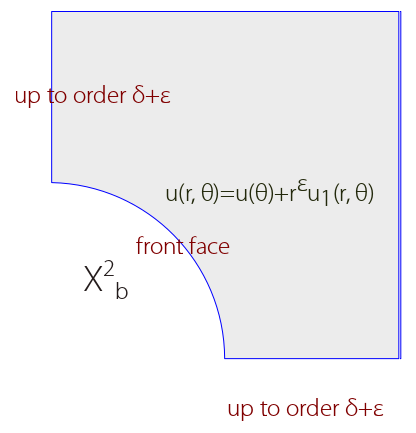
\includegraphics[width=60mm]{drawing71.png}
\end{center}
\definition 
Let $\alpha>0$. The space $\SOA$ consists of conormal distributions which vanishes up to order $\alpha+\delta$ near the two boundaries, and is of the form
\begin{align}
\mu=\mu_0(\theta)+r\mu_1(\theta)+\cdots +r^{\alpha}u_{k+1}(r,\theta)
\end{align}
such that $\forall i, 0\le i\le k$, we have $\mu_i(\theta)\in \theta^{\alpha+\delta}(\frac{\pi}{2}-\theta)^{\alpha+\delta}h$, $h\in \mathcal{S}^{0}([0,\frac{\pi}{2}])$. 

\discussion 
The previous definition is the special case when $0<\epsilon<1$.  

\definition 
We define $\Psi^{-\infty, \alpha}_{b}(X)$ as conormal distributions with kernels in the space $\SOA*\Omega_{b, R}$. 

\definition We can also define $\Psi^{m,\alpha}_{b}(X)$ as conormal distributions with kernels in the space $\Psi^{m,\alpha}_{b}(X)$. 

\example 
Let $\phi\in C^{\infty}_{c}(X^2_b, \Delta_b)$ and $\phi K\in S^{0,\alpha}_{ff}(X^2_b)$. Or if $\phi\in C^{\alpha}_{c}(X^2_b)$. In either case $\phi$ is supported on a neighborhood $\mathcal{U}\cong \R^{n,k}_{r, y}\times \R^{n}_{z}$ with $\Delta_b=\R^{n,k}\times \{0\}$. Then we have
\begin{align}
\phi K=\int e^{iz\cdot \xi}a(r,\xi)d\xi\otimes \mu_{R}, \mu\in \Omega_{b, R}
\end{align}
and we have 
\begin{align}
a(r,\xi)=\sum^{k}_{l=0}r^{l}a_{l}(y,\xi)+r^{\alpha}a_{k+1}(r, y,\xi), k=[\alpha], a_{l}(y,\xi)\in \mathcal{S}^{m}, a_{k+1}(r,y,\xi)\in C^{\infty}
\end{align}
where by definition $a_{l}(r, y, \xi) \in \mathcal{S}^{m}$ means
\begin{align}
|\partial_{y}^{\beta}\partial_{\xi}^{\alpha}a_{k+1}(r,y,\xi)|\le C_{\alpha, \beta}(1+|\xi|)^{m-|\alpha|}, C_{\alpha,\beta}>0
\end{align}

\example
Let $X\cong [0,1)_{x}\times Y$. Then $X^2=[0,1)^2\times Y^2$ and $X^{2}_{b}\cong \R^{2,2}\times Y^2$. In this case the coordinate chart $\mathcal{U}\cong [0,1)_{r}\times \R^{n-1}_{y}\times \R^{n}_z$, where $r=x, z_1=\log(\frac{x}{x'}), \omega=y-y'$. Here $(y,\omega)=(y, y-y')$ are local coordinates on $Y\times Y$. Then $(r,y,z)$ where $z=(z_1, \omega)$ are the coordinates on $[0,1)^{2}_{b}\times Y^2$, with $\Delta=\{z=0\}$. See the graph:

\begin{center}
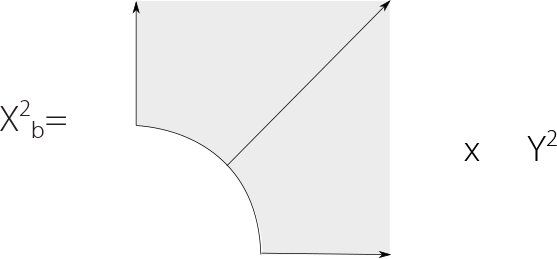
\includegraphics[width=100mm]{drawing84.png}
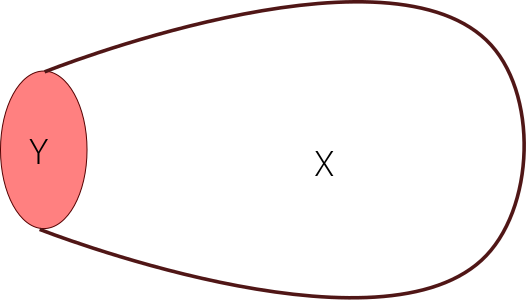
\includegraphics[width=100mm]{drawing83.png}
\end{center}

\example 
Compare with the case where $M$ is  a closed manifold with local coordinates, $x$, then $(x-x', x)$ are local coordinates on $M^2$ with $z=x'-x$, and $\Delta=\{z=0\}$. 

\definition 
The $\textbf{small calculus}$ of order $m\in \R$ is 
\begin{align}
\Psi^{m}_{b}(X)=\bigcap_{\alpha>0}\Psi^{m,\alpha}_{b}(X)
\end{align}

\theorem 
A kernel $K$ belongs to $\Psi^{m}_{b}$ if and only if (omitting density factors):
+
$\phi K\in C^{\infty}(X^b_2)$ and $\phi K$ vanishes with infinity order at left and right boundaries. 
+
For all $\phi\in C^{\infty}_{c}(X^b_2)$ near $\Delta_b$, we have that
\begin{align}
\phi K=\int e^{iz\cdot \xi}a(r,y,\xi)d\xi, a(r,y,\xi)\in S^{m}(\R^{n,k}_{r,y}; \R^{n})
\end{align}
and $a(r,y,\xi)$ is smooth in $y$. In other words $a(r,y,\xi)$ for fixed $r,\xi$ is in $S^{0}(Y)$. 

\proof
+
To show this it suffice to notice that
\begin{align}
\bigcap_{\alpha>0}\SOA=\{\mu\in C^{\infty}(X^2)|\mu\equiv 0 \textrm{  via Taylor series at left/right boundaries} \}
\end{align}
which follows as it has to vanish up to order $\delta+\alpha$ for all $\alpha>0$. This implies it vanishes for all orders of $\alpha$. Hence must be $0$ of infinite order. Indeed we have the following picture:
\begin{center}
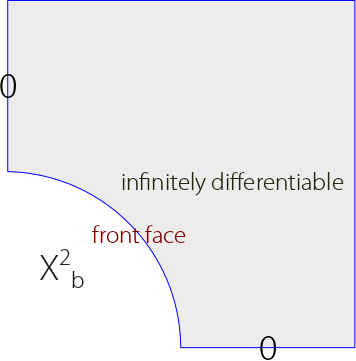
\includegraphics[width=60mm]{drawing72.png}
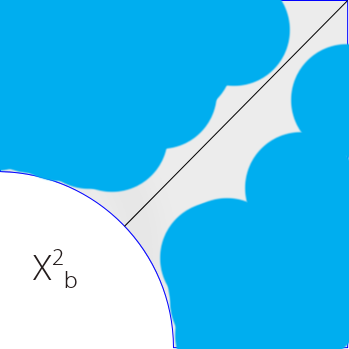
\includegraphics[width=60mm]{drawing73.png}
\end{center}
To show the desired smoothness near the front face we notice that we actually have an infinite Taylor expansion near the d. So the result follows. 
+
This follows by
\begin{align}
\bigcap_{\alpha>0}\mathcal{S}^{m,\alpha}((0,1];\R^{n})=\mathcal{S}^{m}((0,1]_{r},\R^{n})
\end{align}

\qed 

\corollary 
$b$-differential operators are in small calculus. So we have
\begin{align}
Diff^{m}_b(X)\subseteq \Psi^{m}_{b}(X)
\end{align} 
\proof
This follows since $b$-differential operators has to vanish up to infinite order near the boundary, and by definition they are smooth away from the diagonal. 
\qed

\theorem 
We have 
\begin{align}
\Psi^{m}_{b}(X)\cdot \Psi^{m'}_b(X)\subset \Psi^{m+m'}_b(X)
\end{align}
\proof
This follows from composition theorem of conormal distributions we did last semester. 
\qed  

\discussion 
Let us consider Theorem 2 in more detail.  Let $A\in \Psi^{m}_b(X)$, if $\mathcal{U}\cong \R^{n,1}_{r}\times \R^{n}_{z}$ is a ``coordinate patch'' on $X^2_b$ with $\mathcal{U}\cap \Delta_b\cong \{z=0\}$. then we have 
\begin{align}
\phi \mu=\int e^{iz\cdot \xi}a(r ,y,\xi)d\xi\otimes \frac{dx'}{x'}, z=\log(\frac{x}{x'})
\end{align}
From last semester, we have 
\begin{align}
\sigma_m(A)(r,\xi)=[a(r,\xi)]d\xi\otimes \frac{dx'}{x'}dy, [a(r, y,\xi)]\in \mathcal{S}^{m}(\R^{n,1};\R^{n})/\mathcal{S}^{m-1}(\R^{n-1}, \R^{n})
\end{align}
We note that here $\xi$ belong to the conormal space of the diagonal:
\definition  
\begin{align}
N^{*}(\Delta_b)=\{\xi \in T^{*}_{p}X^2_b|\xi\equiv 0 \textrm{  on  } T_{p}\Delta_b \}
\end{align}
and we try to think of $d\xi$ as the dual of $dz$.  \textbf{We note that $dz$ spans $N^{*}_p(\Delta_b)$ because $dz\equiv 0$ on $\partial_{r}, \partial_{y_i}$, which spans $T_p(\Delta_b)$}.The principal symbol $\sigma_{m}(A)(r,y,\xi)$ can thus be viewed in the cotangent space, which we will discuss later. 

To be more explicit, we identify $\xi=(\xi_1\cdots \xi_n)\in \R^{n}$ with $\sum \xi_i dz_i\in N^{*}(\Delta_b)$ as $dz_i$ are the basis vectors. 


\theorem 
The map
\begin{align}
\forall \alpha\in T^{*}X, \alpha\rightarrow \pi_{L}^{*}\alpha-\pi_{R}^{*}\alpha\in N^{*}_p(\Delta)
\end{align}
on the interior of $X$ extends to a map 
\begin{align}
{}^{b}T^{*}X\xrightarrow{D} N^{*}(\Delta_b)
\end{align}
\proof 
We need to look at $dz_1\cdots dz_n$.  We recall that $z_{1}=\log(\frac{x}{x'}), z_2=y_1-y_1'\cdots z_n=y_{n-1}-y_{n-1}'$. Thus we can write
\begin{align}
z=(z_1,w), w=y-y'
\end{align}
as well as
\begin{align}
dz_1=\frac{dx}{x}-\frac{dx'}{x'}=\pi_{L}^{*}(\frac{dx}{x})-\pi^{*}_{R}(\frac{dx}{x}), dz_k=dy_{k-1}-dy_{k-1}'=\pi^{*}(dy_k)-\pi^{*}_{k}(dy_k)
\end{align}
where by definition $x_{1}\partial_{1}, y_{k}\partial_{k}$ spans $\BTX$. The map thus gives a 1-1 correspondence $dz_k=D(\partial_{k})$. 

\qed 

\discussion 
We now go back to the principal symbol:
\begin{align}
\sigma_m(A)(r,\xi)=[a(r,\xi)]d\xi\otimes \frac{dx'}{x'   }dy'
\end{align}
whereas we recall that
\begin{align}
d\xi=|d\xi_1\wedge \cdots \wedge d\xi_n|\in \Omega(N_p(\Delta_b))\cong [(dz_1)^{*}\cdots \wedge (dz_{n})^{*}]
\end{align}
Now recall that $d\xi_k=(dz_{k})^{*}=\partial_{z_k}$. Then we have 
\begin{align}
d\xi&=|d\xi_1\wedge \cdots \wedge d\xi_n|\\
&=|(dz_1)^{*}\wedge \cdots (dz_n)^{*}|\\
&\in \Omega (N^{*}(\Delta_b))^{*}\\
&\in \Omega^{-1}(N^{*}(\Delta_b))\\
&\cong\Omega^{-1}({}^{b}T^{*}X)
\end{align}
$\therefore$  We have $d\xi\otimes (\frac{dx'}{x'}dy)\in \Omega^{-1}({}^{b}T^{*}X)\otimes \Omega({}^{b}T^{*}X)=\C$.  In fact, we have
\begin{align}
d\xi\otimes \frac{dx'}{x'}dy'&=|\alpha_1^{*}\wedge \cdots \wedge \alpha_{n}^{*}|\otimes |\alpha_1\wedge \cdots \wedge \alpha_n|=1
\end{align}
Therefore we can view $\sigma_{m}(A)\in \mathcal{S}^{m}({}^{b}T^{*}X)$. Overall we have the map given by
\begin{align}
\alpha\rightarrow \pi_L^{*}(\alpha)-\pi_{R}^{*}(\alpha)\in (T^{*}X)^2=T^{*}X\oplus T^{*}X
\end{align}

\discussion 
Geometrically we have the following picture: 
\begin{center}
\includegraphics[width=190mm]{drawing74.png}
\end{center}
The picture is better than the words and I encourage everyone to look at the picture. Thanks for Kunal Sharma for the photo! More generally, if $A\in \Psi^{m,\alpha}(X)$, then $\sigma_{m}(A)\in \mathcal{S}^{0,\alpha,m}({}^{b}T^{*}X)=\mathcal{S}^{0,\alpha,[m]}({}^{b}T^{*}X)/\mathcal{S}^{0,\alpha,m-1}({}^{b}T^{*}X)$.

\definition 
$a\in \Psi^{m, \alpha}_b$ is elliptic if there exists $b\in \mathcal{S}^{0,\alpha,[-m]}({}^{b}T^{*}X)$ such that $$[ab]=1$$ in $S^{0,\alpha,[0]}({}^{b}T^{*}X)$. In other words, $ab-1\in \mathcal{S}^{0,\alpha, -1}({}^{b}T^{*}X)$. 

\discussion 
If we are working with small-$b$-calculus, then we can get rid of $(0,\alpha)$s. If $A$ is in small calculus, $A$ is elliptic if there exists $b\in \mathcal{S}^{-m}({}^{b}T^{*}X)$ such that $ab-1\in \mathcal{S}^{-1}({}^{b}T^{*}X)$. Similar to the case of closed manifolds, we have the following three theorems:

\theorem 
For all $m\in \R$, we have exact sequence
\begin{align}
0\rightarrow \Psi^{m-1,\alpha}_{b}\rightarrow \Psi^{m,\alpha}_{b}\rightarrow \mathcal{S}^{0,\alpha, [m]}({}^{b}T^{*}X)\rightarrow 0
\end{align}

\theorem 
If $A$ is elliptic and $A\in \Psi_{b}^{m,\alpha}(X)$. Then there exists $B\in \Psi^{-m, \alpha}_{b}(X)$ such that 
\begin{align}
AB=Id-R_1, BA=Id-R_2\in \Psi^{-\infty, \alpha}_b(X)
\end{align}
\proof
The proof of the left/right paramatrix is exactly the same as the closed manifold case. We fix $\alpha$ and cut-off $A$ near the boundary, which converts it to the closed manifold case. Then we can use continuity principle to show $AB, BA$ belongs to the desired class of conormal distributions. 
\qed 

\noindent 
We have analogous theorem for small calculus:
\theorem 
If $A$ is elliptic and $A\in \Psi_{b}^{m}(X)$. Then there exists $B\in \Psi^{-m}_{b}(X)$ such that 
\begin{align}
AB=Id-R_1, BA=Id-R_2\in \Psi^{-\infty}_b(X)
\end{align}

\discussion 
Let us remind ourselves of the main issue, namely how to show an operator is Fredholm. Recall that in the closed manifold case, we showed it using Stone-Weistrauss theorem by constructing an $F$, which is an approximation of $R_1$, such that $|-R_1+F|$ is small. The strategy in this is case would be to invent $F$ directly. There will be subtle issues we want to address. 

Assuming that $AB=Id-R_1$, let $B'=(Id-R_1+F)^{-1}$ and assuming $|R_1-F|$ is small. Then we have 
\begin{align}
AB'=Id-F', F'=F\circ (Id-R_1+F)^{-1}
\end{align}
then $A$ would be Fredholm because $F'$ is still a finite rank operator. But this assumes we can find $R_1$ close to $F$. We want to carry out Stone-Weistrauss program for $R_1$. If $F$ exists, we know $F\in C^{\infty}(X\times X)$, therefore $F=\sum \phi_i \psi_i(x,x')$, where after omitting the density factors we have $\phi_i, \psi_i\in C^{\infty}(X)$.  For us to use Stone-Weistrauss, we need to have at least $R_1\in C^{0}(X\times X)$. But this is unfortunately not true: 

\theorem
We have the following equivalence:
\begin{align}
R\in C^{0}(X^2)\leftrightarrow R|_{ff}=\{ \mu\in C^{\infty}(X^2_b)|\mu\equiv 0 \textrm{ on left and right boundary} \}
\end{align}
\proof
The proof is quite easy. We have the following geometrical way to visualize it. For $R$ off the front face, it must be living in $X^2$. Therefore there exists $v\in C^{0}(X^2)$, such that $R=v$ in $X/\partial X$. We now have the following picture of $X^2_b$ in polar coordinates:
\begin{center}
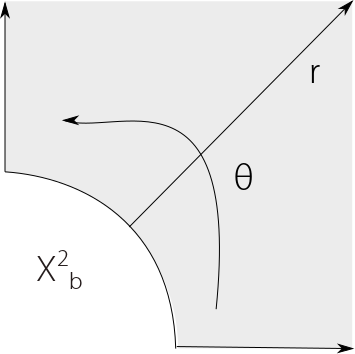
\includegraphics[width=60mm]{drawing75.png}
\end{center}
Suppose $\mu \in C^{\infty}([0,1)_{r}\times [0,\frac{\pi}{2})_{\theta}$ and $\mu \equiv 0$ at $\theta=0/\theta=\frac{\pi}{2}$ with $r=\sqrt{x^2+x'^2}$ and $\theta=\tan^{-1}(\frac{x'}{x})$. This defines a $v$ on $X^2$ except on point $(0,0)$ via
\begin{align}
v(x,x')=u(\sqrt{x^2+x'^2}, \tan^{-1}(\frac{x'}{x}))
\end{align}
\indent The question is when $v$ is a continuous function on $X^2$. Since $v$ is continuous everywhere else,  we are really concerned under what conditions $v$ is continuous up to $0$. 
\begin{center}
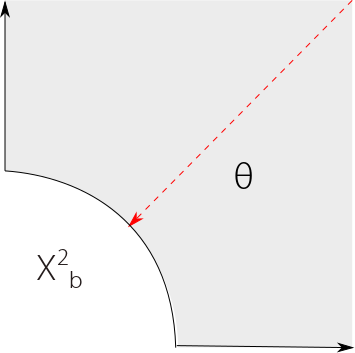
\includegraphics[width=60mm]{drawing76.png}
\end{center}
We observe that under red radial lines like this, we would have
\begin{align}
\lim_{(x,x')\rightarrow (0,0)}v(x,x')=\lim_{r\rightarrow 0}u(r,\theta)=\mu(0,\theta)
\end{align}
Therefore if $\lim_{(x,x')}v(x,x')=0$, then $u(0,\theta)=0$ for all $\theta$. This would imply that $\mu$ restricted on the front face is zero.

Conversely, if $\mu(r,\theta)=0,\forall \theta$, then by uniform continuity for all $\epsilon>0$, there exists $\delta>0$ such that if $0\le r<\delta$, then $|\mu(r,\theta)|<\epsilon$. Therefore if $r=\sqrt{x^2+x'^2}<\delta$, then $v(x,x')=u(\sqrt{x^2+x'^2}, \tan^{-1}(\frac{x'}{x}))$ would be less than $\epsilon$ as well. Thus by taking limits we have $\lim_{(x,x')\rightarrow 0}u=0$ as desired. 

Our conclusion is that $R_1$ restricted to the front face will be of great importance. 
\qed 

\discussion 
In fact, it is an example of a so-called $\textit{normal operator}$. From what we discussed earlier, the restriction to front face is the obstruction to an elliptic $b$-operator to be Fredholm. Note that we may introduce $\log$-coordinates as usual, in this case $z_1=\log(\frac{x}{x'})$.  We have the following picture:
\begin{center}
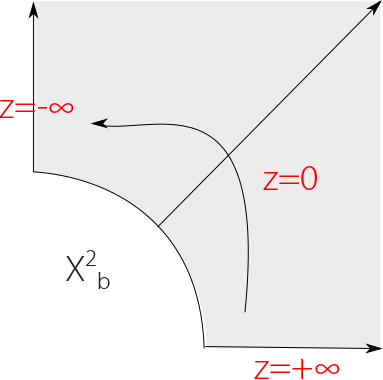
\includegraphics[width=60mm]{drawing77.png}
\end{center}
We know that near the boundary, the front face is differeomorphic to $\R\times Y^2$. The vanishing conditions can be translated to
\begin{align}
R_1(z,y,y') \textrm{vanishes as } |z|\rightarrow +\infty
\end{align}
Instead of working with $R_1$ directly, we can look at its Fourier transform:
\begin{align}
 \widehat{R}_{1}(\tau)=\int e^{-iz\cdot \tau}R(z,y,y')dz
\end{align}
We claim that $ \widehat{R}_1(\tau)=0$ if and only if $R$'s restriction on the front face is zero. 

\definition 
$ \widehat{R}_1(\tau)$ defined earlier is an example of $\textbf{normal operator}$. In Melrose's notation it is often denoted by $ \widehat{R}(\tau)=I(R)(\tau)=N(R)(\tau)$. 

\discussion 
Since $R_1$ vanishes at the left and right boundary, we conclude $R_1$ actually vanishes when $|z|\rightarrow \infty$ in (35). We note that actually more is true. For all $\alpha>0$, we have 
 \begin{align}
R(0,z,y,y')\in O(e^{\tau z}), z\rightarrow -\infty, R(0,z,y,y')\in O(e^{-\tau z}), z\rightarrow +\infty
 \end{align}
by our discussion in earlier lectures of super-exponential decay. We also note that 
 \begin{align}
 \widehat{R}_1(\tau)\in C^{\infty}(Y\times Y)\subseteq \Psi^{-\infty}(Y\times Y), Y=\partial X
\end{align}
Now locally we can write 
 \begin{align}
R_1=\int e^{iz\cdot \tau+i(y'-y)\eta}a(r,\tau,\eta)d\tau d\eta\otimes \frac{dx'}{x'}dy', a\in \mathcal{S}^{-\infty}(\R^{n,1}; \R^{n})
 \end{align}
 and by restricting on the front face we have (ignoring the harmless density factor)
 \begin{align}
  R_1|_{ff}=\int e^{iz\cdot \tau+i(y-y')\eta}a(0,y,\tau,\eta)d\tau d\eta\otimes dy'
 \end{align}
 and its Fourier transform is given by
  \begin{align}
 \widehat{R}_1(\tau)=\int e^{i(y-y')\eta}a(0,y,\tau,\eta)d\eta\otimes dy'
  \end{align}
 where
 \begin{align}
 a\in \mathcal{S}^{-\infty}(\R^{n-1}; \R\times \R^{n-1}_y)
 \end{align}
 The motivation of working with the Fourier transform is now clear: we want to remove the $e^{iz\cdot \tau}$ part in (39), which is almost a nuisance. Then we can focus on the $Y$ factor. We thus think $\R_1$ as parametrized by $\tau$ and is a $\Psi DO$ in $\tau$. 
 
 \discussion 
 We can define normal operators for $\Psi^{m,\alpha}_{b}(X)$ in the same exact way. Let $A\in \Psi^{m, \alpha}_{b}(X)$. Then $A$ has a kernel $u$, see the graph: 
 \begin{center}
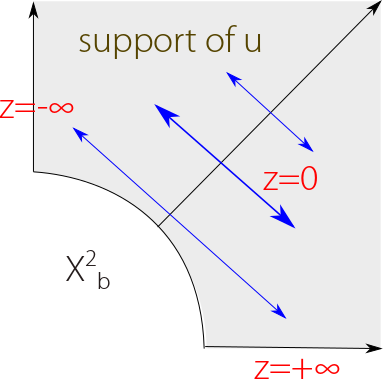
\includegraphics[width=60mm]{drawing78.png}
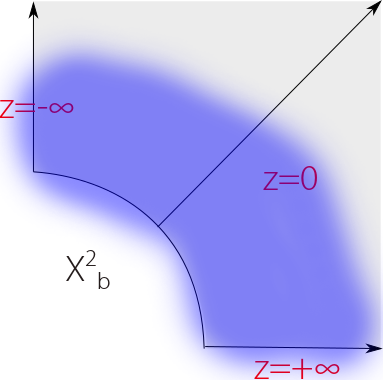
\includegraphics[width=60mm]{drawing79.png}
 \end{center}
 Locally we have 
\begin{align}
A=\mu\frac{dx'}{x'}, \mu=\int e^{iz\cdot \tau+i(y'-y)\eta}a(r,\tau,\eta)d\tau d\eta dy'
\end{align}
Then we have
\begin{align}
\mu|_{ff}=\int e^{iz\cdot \tau+i(y'-y)\eta}a(0,\tau,\eta)d\tau d\eta dy'
\end{align}
 as well as
 \begin{align}
 \widehat{A}(\tau)= \widehat{A|_{ff}}(\tau)=\int e^{(y-y')\cdot \eta} a(0,y, \tau, \eta)d\eta\otimes dy'
 \end{align}
 Since we know that
\begin{align}
 a(r,y,\tau, y)\in S^{m}(\R^{n,1})\leftrightarrow |\partial^{\beta}_{y}\partial^{\alpha}_{\tau}\partial^{\gamma}_{\eta}a(0,y, \tau, \eta)\le (1+|\tau|+|\eta|)^{m-|\gamma|-|\alpha|}
\end{align}
 We observe that by (46), for all $\tau \in \R$,  $ \widehat{A}(\tau)\in \Psi^{m}(Y)$. As a conclusion we note that $ \widehat{A}(\tau)$ is a $\Psi DO$ depending on the parameter $\tau\in \R$. For all $\alpha>0$, we have
 \begin{align}
 \widehat{A}(\tau): C^{\alpha}(Y)\rightarrow C^{\alpha}(Y)
 \end{align}
 We now let $\phi\in C^{\infty}(Y)$ and extend $\phi$ to $X$ in any way we desired. So there exists $\tilde{\phi}\in C^{\infty}(X)$ such that $\tilde{\phi}_{\partial X=Y}=\phi$. Now we have the following theorem:
 
 \theorem 
 For all $\tau \in \R$, we have
  \begin{align}
 \widehat{A}(\tau)\phi=x^{-i\tau}Ax^{i\tau}\tilde{\phi}|_{x=0}
  \end{align}
 \proof
 We claim the theorem is really trivial. We shall prove it via continuity principle:
  \begin{center}
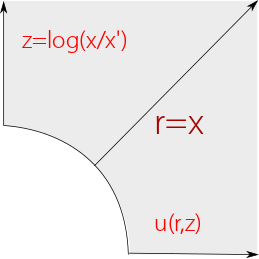
\includegraphics[width=60mm]{drawing85.png}
  \end{center}
 We have
\begin{align}
(x^{-i\tau}Ax^{i\tau}\psi)&=\int \mu(x,\log(\frac{x}{x'}))\tilde{\phi}(x')\frac{dx}{x'}\\
&=\int x^{-i\tau}\mu(x,\log(\frac{x}{x'}))x'^{i\tau}\tilde{\phi}(x')\frac{dx}{x'}\\
&=\int e^{-iz\cdot \tau}\mu(x,z)\tilde{\phi}(xe^{-z})dz, \frac{x}{x'}=e^{z}\\
&\rightarrow \int e^{-iz\cdot \tau}\mu(0,z)\tilde{\phi}(x=0)dz,  \textrm{restricting to the front face where } x=0 \\
&= \widehat{A}(\tau)\phi \textrm{by  Fourier inversion formula}
\end{align}
where we might have implicitly used the fact from Dirac distribution in the last step: 
\begin{align}
f(0)=\int e^{-iz\cdot \xi}\widehat{f}(\xi)d\xi|_{z=0}=\int \int e^{iz\cdot \xi}f(z)dzd\xi
\end{align}
\remark
I feel the density factor in (49) should really be $\frac{dx'}{x'}$, but then we would face an essential difficulty as we cannot get from (50) to (51) easily. Similarly I think (52) to (53) takes some work. I think $\tilde{\phi},\phi$ both cannot take values in $\tau$. 
\discussion 
Now as a corollary we have:
\corollary
\begin{align}
\widehat{A\circ B}=\widehat{A}(\tau)\circ \widehat{B}(\tau)
\end{align}
\proof
This is clear because choosing $\psi_{\partial X}=\phi$, we have:
\begin{align}
\widehat{A\circ B}(\tau)\phi&=x^{-i\tau}A\circ B x^{i\tau}\psi|_{x=0}\\
&=x^{-i\tau}Ax^{i\tau}\circ (x^{-i\tau}Bx^{i\tau}\psi)|_{x=0}\\
&= \widehat{A}(\tau)\circ (x^{-i\tau}B x^{i\tau}\psi)|_{x=0}\\
&=\widehat{A}(\tau)\circ \widehat{B}(\tau)\phi 
\end{align}

\example Let us consider the canonical example. Let 
\begin{align}
D=\frac{1}{i}\sigma(x\partial_x+D_y), D\in Diff^{1}_b(X)
\end{align}
Then we have
\begin{align}
 \widehat{D}(t)\phi&=x^{-i\tau}D x^{i\tau}\psi|_{x=0}\\
&=\frac{1}{i}\sigma(i\tau+D_{y})\phi
\end{align}
Therefore
\begin{align}
 \widehat{D}=\frac{1}{i}\sigma(\i\tau+D_{y})
\end{align}
as desired. 

\discussion 
Our plan would be to let $AB=I-R_1$, and use some $S\in \Psi^{-\infty}_b$ as a correction factor. We want $S|_{ff}=0$, which is equivalent to $\widehat{S}(\tau)=0,\forall \tau\in \R$.  This way we can conclude it is Fredholm. We now assume that $\widehat{A}(\tau)^{-1}$ exists for all $\tau\in \R$, then we suppose that we can find $B_1\in \Psi^{-m,\alpha}_{b}$ such that $ \widehat{B}_1= \widehat{A}(\tau)^{-1}$. Now we let 
\begin{align}
S=R-A\circ B_1\circ R_1, B_2=B+B_1\circ R
\end{align}
we have
\begin{align}
A\circ B_2&=A\circ B+A\circ B_1\circ R_1\\
&=I-R_1+A\circ B_1\circ R_1\\
&=I-S
\end{align}
But we note that
\begin{align}
 \widehat{S}(\tau)&= \widehat{R}_1(\tau)- \widehat{A}(\tau)\circ  \widehat{B}_1(\tau)\circ  \widehat{R}_1(\tau)\\
&=0\\
\end{align}
and we may conclude that $A$ is Fredholm after all!
\corollary 
We assert that $ \widehat{A}(\tau)^{-1}$ does exist for $\tau$ large. The remaining issues to address are whether $ \widehat{A}(\tau)^{-1}$ is holomorphic in $\tau$. And we would need analytical Fredholm theory to address questions like
\begin{align}
 \widehat{A}(\tau) \widehat{B}(\tau)=I- \widehat{R}(\tau), E=\int  \widehat{D}(\tau)^{-1}
\end{align}

\section{Lecture 12: The normal operator}
We keep discussing the normal operator. Let $K_A$ be a conormal distribution on $X_2^b$. Then by restricting to the front face we have $\textbf{front face}\cong \R\times Y\times Y$. Now we have
\begin{align}
 \widehat{A}(\tau)=\int_{\R}e^{-iz\cdot \tau}K_{A|\textbf{front face}}(z)dz, K_{A}=\mu*\frac{dx'}{x'}
\end{align}
where we omitted the density factor. 
 \begin{center}
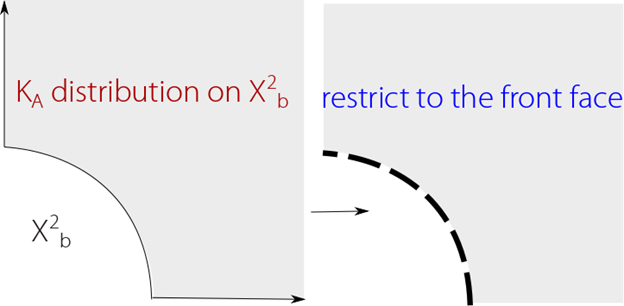
\includegraphics[width=120mm]{drawing82.png}
 \end{center}
Last time we showed that for
\begin{align}
 \widehat{A}(\tau):C^{\infty}(Y)\rightarrow C^{\infty}(Y)
\end{align}
we have
\begin{align}
 \widehat{A}(\tau)\phi=x^{-it}Ax^{it}\tilde{\phi}|_{x=0},  \widehat{\phi}\in C^{\infty}(X),  \widehat{\phi}|_{\partial X=Y}=\phi
\end{align}

\example 
Let $A\in Diff^{m}_b(X)$, then we have $A=\sum_{|\alpha|+|\beta|\le m}^{m}(x\partial_{x})^{\alpha}\partial_{y}^{\beta}$, then $ \widehat{A}(\tau)=\sum_{|\alpha|+|\beta|\le m}(i\tau)^{\alpha}(\partial_{y})^{\beta}$. 

\example 
Let $D$ be a generalized Dirac operator. Then we have $D=\frac{1}{i}\sigma(x\partial_x+D_{y})$, with $ \widehat{D}(\tau)=\frac{1}{i}\sigma(i\tau+D_y)$. 

\example 
Assume $K_{A}$ as the kernel of conormal distribution is supported near $\Delta_b$, $A\in \Psi^{m}_b(X)$. Then we have
\begin{align}
K_A=\int e^{iz\cdot \tau}a(r,z,\tau)d\tau
\end{align}
by definition of conormal distributions, where $a(r,z,\tau)\in S^{m}(\R^{n,1};\R^{n})$ in local coordinates in $(r,z)$. In reality we really need to include the density factors and we are working with $S^{m}([0,1)_{r}\times \R_{z},\R)$. This means we actually have
\begin{align}
K=\int e^{iz\cdot \xi}a(r,z, 
\xi)d\xi\frac{dx'}{x'}dy', z=(z,y,y'), z_1=\log(\frac{x}{x'}), \xi=(\tau, \eta)
\end{align}
which is again just an abbreviation of
\begin{align}
K_{A}=\int e^{iz\cdot \tau+i(y-y')\cdot \eta}a(r,y,z,\tau, \eta)d\tau d\eta  \frac{dx'}{x'}dy'
\end{align}
which is compact supported in $z$. But we all know that no one ever written this way. Now let $u=\int e^{iz\cdot \tau}a(r, z,\tau)d\tau$. By definition we then have
\begin{align}
\widehat{A}(\tau)&=\widehat{\mu|_{r=0}}(\tau)\\
&=\mu|_{r=0}(e_{\tau}), e_{\tau}(z)=e^{-iz\cdot \tau}
\end{align}
\remark
I think I have trouble with (79). Not sure how we get from (78) to (79). Did we just treat $e_{\tau}$ as a function of $z$ and let $\mu$ evaluate on $e_{\tau}$? 

\discussion 
Note that if we pick up any $\phi\in C^{\infty}_{c}(\R)$ as a cut-off function with $\phi\equiv 1$ on $\textrm{supp} u|_{r=0}$, then we have $\widehat{A}(\tau)=(\mu|_{r=0})(\phi e_{\tau})$ with $\phi e_{\tau}\in C^{\infty}_{c}(\R)$. So $(\mu|_{r=0})(\phi e_{\tau})$ now makes sense. Sine $\phi(z)a(0,z,\xi)=a(0,z,\xi)$ we have 
\begin{align}
 \widehat{A}(\tau)=(\mu|_{r=0})(\phi e_{\tau}), \mu|_{r=0}=\int e^{iz\cdot \tau}a(0,z,\tau)d\tau
\end{align}
Therefore we have
\begin{align}
 \widehat{A}(\tau_0)&=(\mu|_{r=0})(\phi e_{\tau_0})\\
&=\int e^{iz\cdot \tau}\phi(z)e^{-z\cdot \tau_0}a(0,z,\tau)dzd\tau\\
&=\int e^{iz(\tau-\tau_0)}a(0,z,\tau)dzd\tau\\
&=\int \widehat{a}(0,\tau_0-\tau, \tau)d\tau
\end{align}
where by definition
\begin{align}
 \widehat{a}(0,\varrho, \tau)=\int e^{-iz\cdot \varrho}a(0,z,\tau)dz
\end{align}
is the left symbol of $a$ restricted to the front face. 

\discussion
We remind ourselves for this from last semester: For $\mu\in I^{m}(\R^{k}_x\times \R^{n}_z, \R^{k}\times \{0\})$, we have 
\begin{align}
\mu=\int e^{iz\cdot \xi}a(x,z,\xi)d\xi
\end{align}
and we can write it in the left symbol as
\begin{align}
\mu=\int e^{iz\cdot \xi}\tilde{a}(x,\xi)d\xi, \tilde{a}(x,\xi)=\int  \widehat{a}(x,\xi-h,h)dh
\end{align}
this theorem we actually proved last semester. In our case (84) is exactly the left symbol of $\mu$ restricted to the front face. 

We can thus redo what we did via (85) and (86) through the left symbol. We can just re-write using (86) to get 
 \begin{align}
K_A=\int e^{iz\cdot \tau}a(r,\tau)d\tau\frac{dx'}{x'}
 \end{align}
 with a left symbol, then $ \widehat{A}(\tau)=a(0,\tau)$, which should be ``obvious'' because $K_A$ is the inverse Fourier transform of $a(r,\tau)$ in left reduced form when $z=0$. Therefore we have $ \widehat{A}(\tau)$ be the fourier transform of $K_A$ restricted over the front face is just $a(0,\tau)$. 
 
 \discussion 
 In the general case where
\begin{align}
  K_A=\int e^{iz\cdot \tau+i(y'-y)\cdot \eta}a(r,y,\tau, \eta)d\tau d\eta \frac{dx'}{x'} dy'
\end{align}
as well as
\begin{align}
K_{ \widehat{A}}(\tau)=\int e^{i(y-y')\eta}a(0,y,\tau, \eta)d\eta dy'
\end{align}
such that for all $\eta\in \R$, we have $ \widehat{A}(\tau)\in \Psi^{m}(Y)$. Here $a(0,y,\tau, \eta)$ is an abbreviation of $a(r,y,z,\omega,\tau, \eta)$, where 
 $\mu\in I^{m}([0,1)_{r}\times \R^{n-1}_{y}\times \R_{z}\times \R^{n-1}_{\omega}[0,1)\times \R^{n-1}_{y}\times \{0\}\times \{0\})$.

We want to carry out more in depth analysis of the symbol of normal operators. 

\example 
Let $A\in \Psi^{-\infty, \alpha}_{b}(X)$ such that $K_{A}=\mu\frac{dx'}{x'}$ after omitting the density factors. The associated normal operator, by definition is
\begin{align}
K_{\widehat{A}}(\tau)=\int e^{-iz\cdot \tau}(\mu|_{\textrm{front face}})(z)dz
\end{align}
We note that off the front face, we have $X^2\cong [0,1)_{r}\times \R_{z}$.  So we only need to analyze the behavior near the front face:
 \begin{center}
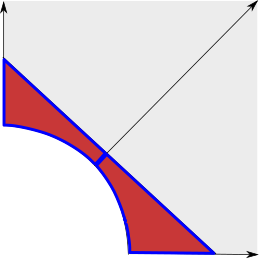
\includegraphics[width=60mm]{drawing87.png}
 \end{center}
 see also the photo provided by Kunal:
 \begin{center}
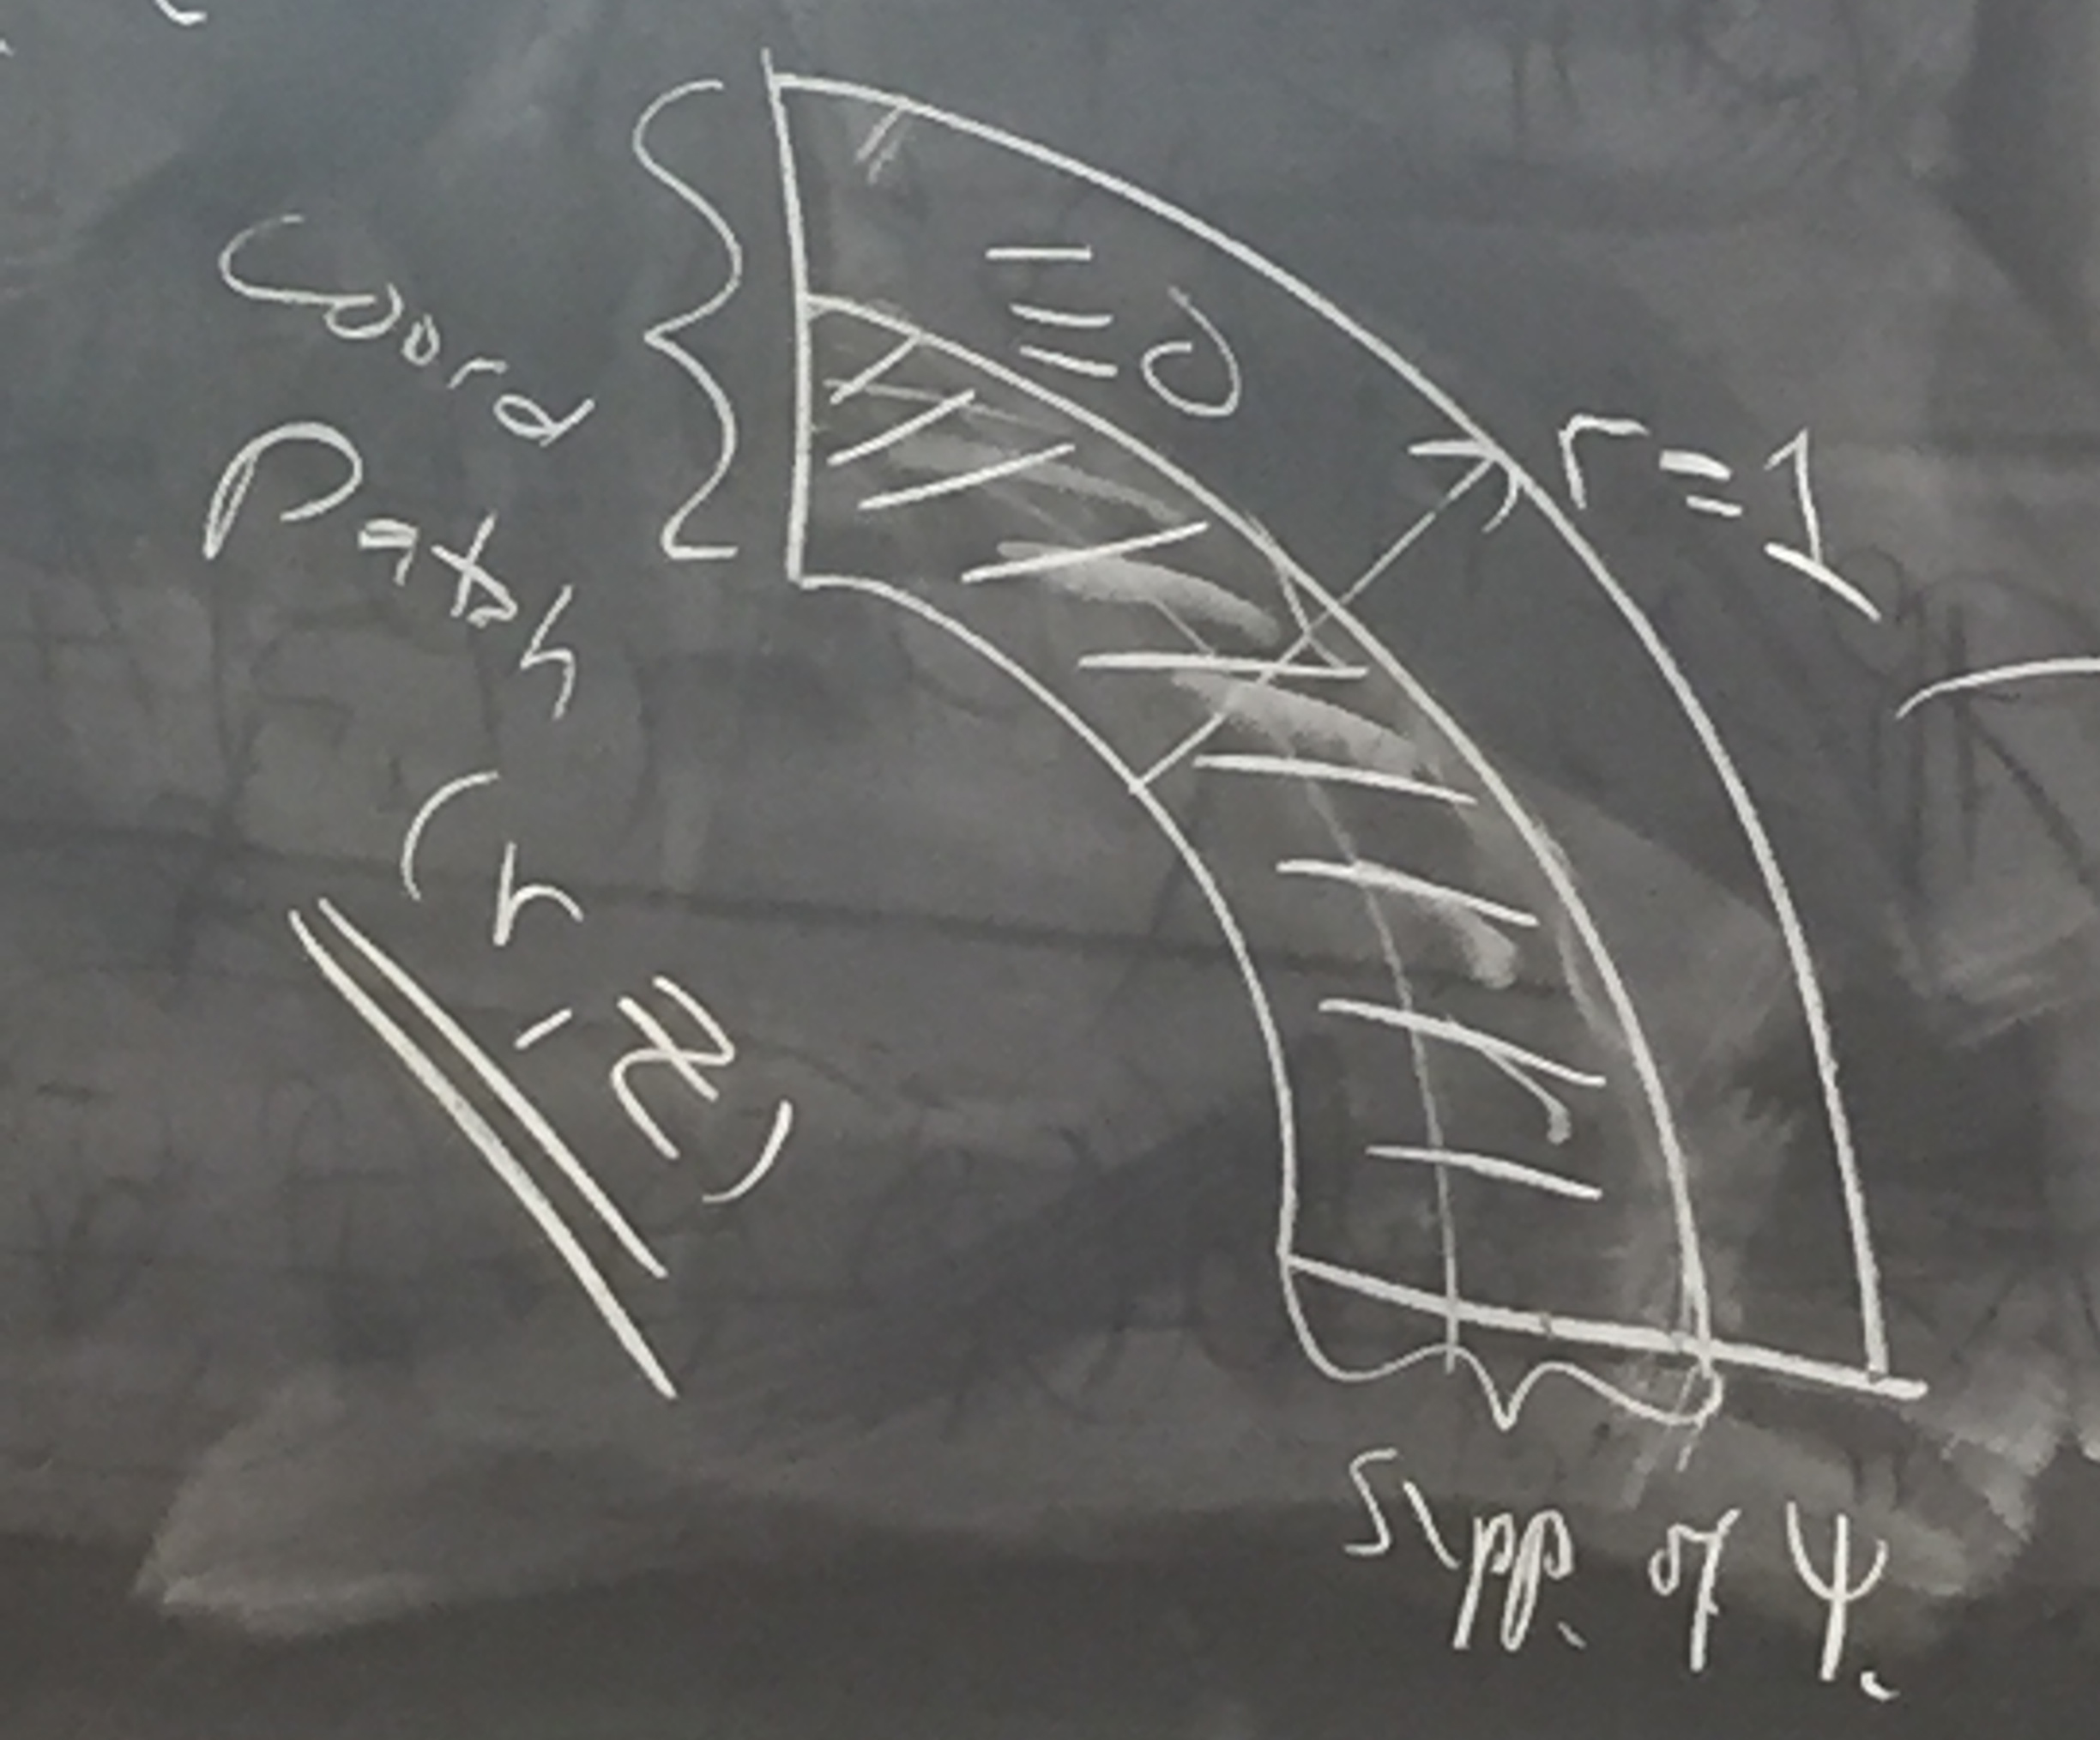
\includegraphics[width=100mm]{drawing97.jpg}
 \end{center}

\remark
I think we chose the cut-off function because we work with the normal operator. Is this true or false?
\discussion 
In particular, near the left boundary, we can take the coordinates 
\begin{align}
\omega_1=x', \omega_2=\frac{x}{x'}, z=\log(\omega_2)
\end{align}
and near the right boundary we can take
\begin{align}
\omega_1=x, \omega_2=\frac{x'}{x}, z=\log(\omega_2^{-1})
\end{align}
 \begin{center}
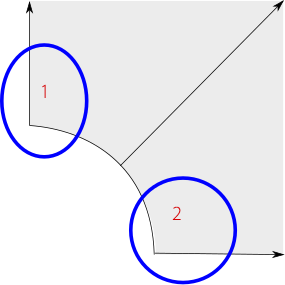
\includegraphics[width=60mm]{drawing88.png}
 \end{center}
Then by definition (2)-(3) of $\Psi^{-\infty,\alpha}_{b}(X)$ there exist some $\delta$ such that
\begin{align}
u|_{\textrm{front face}}=v=O(e^{(\epsilon+\delta)z}), v=O(e^{-(\epsilon+\delta)z})
\end{align}
near but off the left/right boundaries respectively. In other words, now the kernel has exponential decay:
 \begin{center}
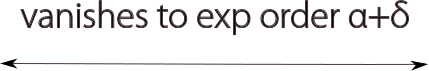
\includegraphics[width=60mm]{drawing89.png}
\end{center}

Let us think about the Fourier transform. We claim that $K_{\widehat{A}}(\tau)$ is in fact a holomorphic functions in $\tau$.  Let $\tau=\tau_1+i\tau_2$, with $\tau_i\in \R$. Then we can write the integral as 
\begin{align}
\int e^{-iz\cdot \tau_1}\cdot e^{\tau_2\cdot z}v(z)dz, z\in \R
\end{align}
We observe that for $|\tau_2|\le \alpha$, we in fact have 
\begin{align}
e^{\tau_2 z}v(z)\in L^{1}(\R)
\end{align}
Indeed, as $z\rightarrow \infty$ we have 
\begin{align}
e^{\tau_2 z}v(z)&=O(e^{\tau_2 z}e^{-\alpha z-\delta z})\\
&=O(e^{-\delta z})
\end{align}
and as $z\rightarrow -\infty$ we have
\begin{align}
e^{\tau_2\cdot z}v(z)&=O(e^{\tau_2\cdot z}e^{(\alpha+\delta)\cdot z})\\
&=O(e^{(\alpha+\delta)\cdot z})
\end{align}
which exponentially decays as $z\rightarrow -\infty$. Therefore  the integral $K_{\widehat{A}}(\tau)$ is well-defined and holomorphic on the horizontal band $\Omega_{\alpha}=|\tau_2|\le \alpha$:
 \begin{center}
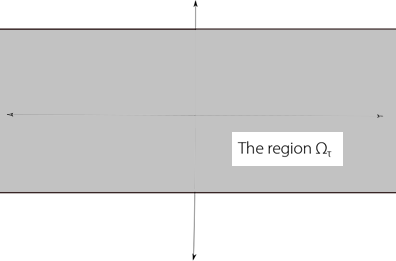
\includegraphics[width=120mm]{drawing90.png}
 \end{center}
This would be important as we go back to $\Psi DO$s!
\remark
I could not really appreciate the importance at this stage. Can Prof.Loya explain? 

\discussion 
We want to go back from the symbol to the operator, which should be possible as long as $e^{\tau_2\cdot z}v(z)\in L^{1}(z), |\tau_2|\le \alpha'$.  Think about it, here is another way to do it. We can write
\begin{align}
K_{A}=\int e^{iz\cdot \tau}a(r,z)d\tau
\end{align}
with $a(r,\tau)$ be the left symbol. Then we have
\begin{align}
K_{ \widehat{A}}(\tau)=a(0,\tau)
\end{align}
and we conclude that $a(0,\tau)$ is defined for $\tau\in \Omega_{\alpha'}$ where $\alpha<\alpha'<\alpha+\delta$. 

\exercise
Show that $a(0,\tau)$ is holomorphic for $\tau \in \Omega_{\alpha'}$ such that for all $\beta, k$ we have 
\begin{align}
|\partial^{\beta}_{\tau}a(0,\tau)|\le C_{\beta, k} (1+|\tau|)^{-k}, \forall \tau\in \Omega_{\alpha'}
\end{align}
\proof
This is basically trying to show Schwartz in $\tau$. But every time we differentiate $a(0,\tau)$ we actually increase $a(r,z)$ by a polynomial type $\tau$ factor. Since we know that $a(r,z)$ is of exponential decay near the two boundaries, $C_{\beta,k}$is bounded for $\beta,k$. This proof is suggested by Adam. 
\qed

\discussion 
This is cool, as now we can do the reverse to go backwards:

\theorem Let $a(\tau)$ be holomorphic in $\Omega_{\alpha'}$, where $\alpha'>0$. Suppose for some $\beta, k$ we have
\begin{align}
|\partial^{\beta}_{\tau}a(\tau)|\le (1+|\tau|)^{-k}, \forall \tau \in \Omega_{\alpha'}
\end{align}
Then given any $\alpha<\alpha'$, there exists $A\in \Psi^{-\infty, \alpha}$ such that $\widehat{A}(\tau)=a(\tau)$.  
\begin{center}
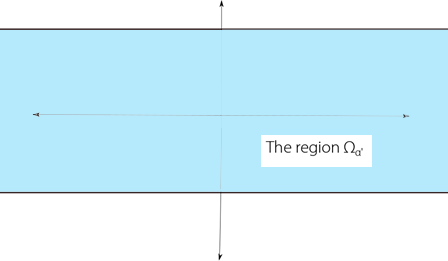
\includegraphics[width=120mm]{drawing91.png}
\end{center}
\proof
In fact, by introducing a cut-off function we have
\begin{align}
A=\phi(r)\int e^{iz\cdot \tau}a(\tau)d\tau\frac{dx'}{x'}, \phi\in C^{\infty}_{c}[0,1), \phi(0)=1
\end{align}
then the kernel
\begin{align}
u(r,z)=\phi(r)\int e^{iz\cdot \tau}a(\tau)d\tau \in S^{0,\alpha}_{\textrm{front face}}(X^2_b)
\end{align}
You can check that in the horizontal band region
\begin{align}
|\textrm{Im} (\alpha)|\le \alpha'
\end{align}
we have 
\begin{align}
u(r,z)&=\int_{\R}e^{iz\cdot (\tau+i\alpha')}a(\tau+i\alpha')d\tau\phi(r)\\
&=e^{-z\cdot \alpha'}\int e^{iz\cdot \tau}a(\tau+i\alpha')\phi(r)d\tau
\end{align}
\begin{center}
 	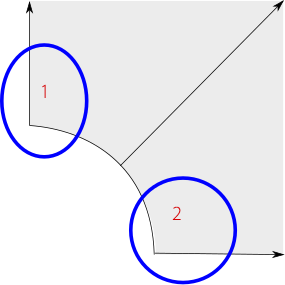
\includegraphics[width=60mm]{drawing88.png}
\end{center}
If we take local coordinates $w_1=x, w_2=\frac{x'}{x}=e^{-z}$, then we have 
\begin{align}
u(r,z)&=e^{-z\cdot \alpha'}\phi(r)\int e^{iz\cdot \tau}a(\tau+i\alpha')d\tau\\
&=\phi(r)w_{2}^{\alpha'}b(w_2)
 \end{align}
 where 
 \begin{align}
b(w_2)=\int w_{2}^{-i\tau}a(\tau+i\alpha')d\tau
 \end{align}
and $a(\tau+i\alpha')$ is Schwartz in $\tau$. Thus $b(w_2)$ is in class $\mathcal{S}^{0}$. 

Similarly over the first coordinate chart we may let $w_1=\frac{x}{x'}, w_2=x'$, and 
 \begin{align}
\mu(r,z)&=\phi(r)\int e^{iz\cdot (\tau-i\alpha')}a(\tau-i\alpha')d\tau\\
&=\phi(r)e^{z\alpha'}*c, c=\int e^{iz\cdot \tau}a(\tau-i\alpha')d\tau\\
&=\phi(r)\omega_2^{\alpha'}c(\omega_2)
 \end{align}
\remark
It seems to me that to show $\Psi^{-\infty,\alpha}_{b}$ we need to show it vanishes up to order $\alpha+\delta$ for some $\delta$. Are we just using the condition $\alpha<\alpha'<\alpha+\delta$ implicitly in our case?

\definition 
 In general we have
 \begin{align}
A=\int e^{iz\cdot \tau+i(y'-y)\cdot \eta}a(r,y,\tau, \eta)d\tau d\eta\frac{dx'}{x'}dy'
 \end{align}
 whereas the associated normal operator is
 \begin{align}
 \widehat{A}(\tau)=\int e^{i(y-y')\cdot \eta}a(0,y,\tau,\eta)d\eta dy'
 \end{align}
 and $a(0, y, \tau, \eta)$ satisfies the following condition:
+
For all $\alpha<\alpha'<\alpha+\delta$, we have $a(0,y,\tau,\eta)$ holomorphic for $\tau\in \Omega_{\alpha'}$. 
+
For all $\beta,\alpha, k$ we have 
 \begin{align}
|\partial^{\beta}_{y}(\partial_{\tau}\partial_{\eta})^{\alpha}a(0,y,\tau,\eta)|\le
C_{\beta, \alpha, k}(1+|\tau|+|\eta|)^{-k}(1+|y|)^{-k}
 \end{align}
In this case we define $A\in \Psi^{-\infty, \alpha}$. 
 
\remark
Missing the last term in the original notes, but this terms seems needed judged from later notes. 

\definition 
We define $A\in  \widehat{\Psi}^{-\infty,\alpha'}$ if and only if $A=\int e^{i(y'-y)\cdot \eta}a(y, z,\eta)d\eta dy'$ with $a\in  \widehat{\mathcal{S}}^{-\infty,\alpha'}$, which we will define later. 
 \discussion
Therefore we have a map
 \begin{align}
\Psi^{-\alpha,a}(X)\xrightarrow{ \widehat{}}\bigcup_{\delta>0}\Psi^{-\infty,\alpha+\delta}
 \end{align}
 
\theorem 
We have a surjective map
 \begin{align}
0\rightarrow r\Psi^{-\infty,\alpha}_{b}(X)\rightarrow \Psi^{-\infty,\alpha}_{b}(X)\rightarrow \bigcup_{\delta>0} \widehat{\Psi}^{-\infty, \delta+\alpha}\rightarrow 0
 \end{align}
 where $r$;s power is the minimum of $(\alpha,1)$, where we used the fact that the expansion on the front face 
 \begin{align}
u(z)=u_{0}(z)+\cdots+ r^{\alpha}\mu_{[\alpha]}(z)
\end{align}
see equation (1), (2) respectively. 
\remark
If I recall correctly we have two cases in this case. Later Prof. Loya modified it again. 
 
\section{Lecture 13: The right function space}
Let us now define $ \widehat{\mathcal{S}}^{-\infty,\alpha}(\R^{n-1})$ rigorously. 
\definition 
It consist of $C^{\infty}$ functions
\begin{align}
\alpha:\R^{n-1}\times \Omega_{\alpha}\times \R^{n-1}\rightarrow \C
\end{align}
such that
+
$a(y,\tau,\eta)$ is holomorphic in $\tau$. 
+
For all $\beta,\alpha,k$ we have
\begin{align}
\alpha:\R^{n-1}\times \Omega_{\alpha}\times \R^{n-1}\rightarrow \C
\end{align}
such that
\begin{align}
 |\partial^{\beta}_{y}(\partial_{\tau}\partial_{\eta})^{\alpha}a(0,y,\tau,\eta)|\le
 C_{\beta, \alpha, k}(1+|\tau|+|\eta|)^{-k}(1+|y|)^{-k}
\end{align}
where $\Omega_{\alpha}=\{\tau\in \C||\textrm{Im}\tau|\le \alpha\}$. 
\begin{center}
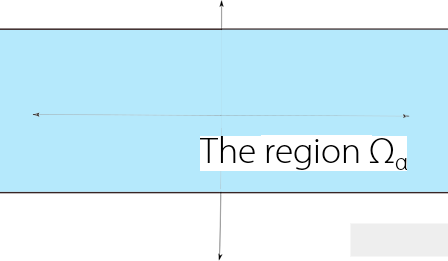
\includegraphics[width=100mm]{drawing92.png}
\end{center}

\discussion 
We thus have the following re-statement of Theorem 9:

\theorem 
The normal operator defines a surjective map
\begin{align}
\Psi^{-\infty,\alpha}(X)\rightarrow \widehat{\Psi}^{-\infty,\alpha}(Y)
\end{align}
where the kernel consists of operators that vanishes on the front face. 

\discussion
The point is that these operators generate the compact operator. Let $A\in \Psi^{-\infty}_{b}(X)$, then $A:S^{0}\rightarrow S^{0}$ is compact(i.e, limit of finite rank operators) if and only if $\ker A$ extends to a continuous function on $X^2$. But as we know this is if only if $A$'s restriction of the front face is $0$, which is our motivation to define $\widehat{A}$. 

The purpose is to go reverse with $K_A$ continuous on $X^2$, then $A$ would be the limit of finite rank operators on $X^2_b$. But this is obvious via Stone-Weistrauss theorem, which says products is dense in the whole space. 

You should think that the fact we are dealing with compact operators implies $K_{A}$ is continuous on $X$. Here we use $\phi_{n}\rightarrow \phi$, such that we have
\begin{align}
x^{i\tau} \widehat{A}x^{-i\tau}\phi_{n}\rightarrow  \widehat{A}\phi
\end{align}
as the space is bounded and we can choose freely a convergent subsequence. 
\remark
I am a bit lost with (126). Another form of continuity principle???

\discussion 
The main thing is for $A\in \Psi^{-\infty, \alpha}(X)$, we have $ \widehat{A}(\tau)$ to be the Fourier transform of $A_{\textrm{front face}}$. Our point is that $ \widehat{A}(\tau)$ is holomorphic and Schwartz for $\tau\in \Omega_{\alpha'}$ for some $\alpha'>\alpha$.  We want to extend what we did earlier to the case of $\Psi^{m,\alpha}_{b}(X)$. The question is what are the corresponding properties of $ \widehat{A}(\tau)$ in this case? 

\definition 
Define $\widehat{\Psi}^{m,\alpha}(Y)$ as families $A(\tau)\in \Psi^{m}(Y)$, such that there exists some $\alpha'>\alpha$ and we locally have
\begin{align}
A=\int e^{i(y-y')\cdot \eta}a(y,\tau,\eta)d\eta dy', a\in \widehat{S}^{m,\alpha'}(\R^{n-1})
\end{align}
We have analogous theorem:

\theorem 
The normal operator defines a map
\begin{align}
\widehat{}:\Psi^{m,\alpha}_{b}(X)\rightarrow \widehat{\Psi}^{m,\alpha}(Y)
\end{align}
whose null space consists of operators $A$ such that $\widehat{A}(\tau)\equiv 0$ for all $\tau\in \R$. 

\proof
We choose local coordinates near the front face. We let $\phi(z)\in C^{\infty}_{c}(\R)$ supported near $z=0$, and $\phi\equiv 1$ near $z=0$. See the image below:
\begin{center}
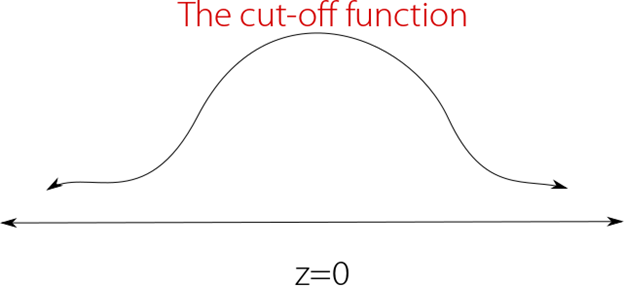
\includegraphics[width=100mm]{drawing80.png}
\end{center}
Now we can write $A=\phi(A)+(1-\phi)A$. As a result we have $\widehat{A}(\tau)=\widehat{\phi A}(\tau)+\widehat{(1-\phi)A}(\tau)$, where because of the domain restrictions the second one belong to $\Psi^{-\infty,\alpha}_{b}(X)$:
\begin{center}
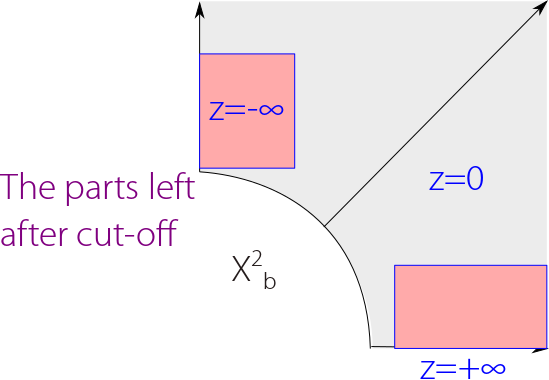
\includegraphics[width=100mm]{drawing81.png}
\end{center}
and the desired decay estimate follows from last theorem. Locally we have
\begin{align}
(1-\phi)A=\int e^{i(y-y')\cdot \eta}a_{1}(y,\tau,\eta)d\eta dy', a_1\in \widehat{S}^{-\infty, \alpha}(\R^{n-1})
\end{align}
So all we need to do is to understand $\widehat{\phi A}(\tau)$. 

+
We know that 
\begin{align}
\phi A=\int e^{iz\cdot \tau}a(r,z,\tau)d\tau
\end{align}
where $a(r,z,\tau)$ is compactly supported in $z$, $C^{\infty}$ in $r,\tau$ and is a symbol of order $m$ in $\tau$. 
+
We know that
\begin{align}
\widehat{\phi A}(\tau)=\tilde{a}(0,\tau)
\end{align}
where $\tilde{a}$ is a left symbol of $\phi A$. We also know that by definition of left symbol we have 
\begin{align}
\tilde{a}(r,\tau)=\int  \widehat{a}(r,r-\zeta, \zeta)d\zeta
\end{align}
where 
\begin{align}
\widehat{a}(r,\zeta,\tau)=\int^{1}_{-1}e^{-iz\cdot \zeta}a(r,z,\tau)dz
\end{align}
where $a(r,z,\tau)$ is compactly supported in $[-1,1]$ by our choice of $\phi(z)$.
Therefore it follows that $\widehat{a}(r,\zeta, \tau)$ is entire in $\zeta\in \C$, since we have 
\begin{align}
\widehat{a}(r,\zeta,\tau)=\int^{1}_{-1}e^{-iz\cdot \zeta}a(r,z,\tau)dz
\end{align}
and differentiation is always well-defined. Thus $ \widehat{a}(r,\zeta, \tau)$ is entire in $\zeta \in \C$. 
\\
Moreover, $ \widehat{a}(r,\zeta,\tau)$ satisfies that for all $\beta,\alpha, \gamma,\gamma>0$ we have 
\begin{align}
|\partial^{\beta}_{\zeta}\partial^{\alpha}_{\tau}\widehat{\alpha}(0,\zeta,\tau)|\le C_{k,\alpha,\beta}(1+|\zeta|)^{-k}(1+|\tau|)^{m-|\alpha|},\forall \zeta\in \Omega_{\delta}, \tau\in \R
\end{align}
where the first part is Schwartz in $\zeta$ and a symbol of order $m$ in $\tau$. In fact, it is easy to show that
\begin{align}
|\partial^{\xi}_{\beta}\partial^{\alpha}_{\tau}\alpha(0,\zeta,\tau)|\le C_{k,\alpha,\beta}(1+|\zeta_1|)^{-k}(1+|\tau|)^{m-|\alpha|}, \forall \zeta\in \Omega_\delta, \tau\in \R
\end{align}
Now for $\zeta\in \Omega_{\delta}$, we have
\begin{align}
\frac{1}{1+\delta}(1+|\zeta|)\le (1+|\zeta_1|)\le (1+|\zeta|)
\end{align}
because we have the simple estimate
\begin{align}
1+|\zeta|&\le (1+\delta)|\zeta_1|+(1+\delta)\\
&=(1+\delta)(1+|\zeta_1|)
\end{align}
which gives us the sharpened inequality (135) above. \\
Therefore by the estimate above we have
\begin{align}
\tilde{a}(0,\tau)=\int \tilde{a}(0,\tau-\zeta,\zeta)d\zeta
\end{align}
is entire in $\xi$ for all $\delta>0$ in the region $\Omega_{\delta}$, and for all $\gamma$ we have
\begin{align}
|\partial^{\gamma}_{\tau}\tilde{a}(0,\tau)|=C_{\gamma}(1+|\tau|)^{m-|\gamma|},\forall \tau\in \Omega_{\delta}
\end{align}
In particular for $\delta<\alpha$, we have
\begin{align}
 \widehat{A}(\tau)=\widehat{\phi A}(\tau)+\widehat{1+\phi}(A)(\tau)\in  \widehat{\Psi}^{m,\alpha}(Y)
\end{align}
as desired. 
\remark
What is the significance of $\delta<\alpha$? Unclear to me. 

+
For surjectivity, we let $B(\tau)\in  \widehat{\Psi}^{m,\alpha}(Y)$. We similarly take coordinates in $(r,z)$ and let $\Psi\in C^{\infty}_{c}([0,1)_{r})$ with $\Psi(0)=1$. To be more explicit, if we have
\begin{align}
B(\tau)&=\int e^{i(y-y')\cdot \eta}b(y,\tau,\eta)d\eta dy'
\end{align}
in local coordinates, then we can define
\begin{align}
A=\int e^{iz\cdot \tau+i(y-y')\cdot \eta}\Psi(r)b(y,\tau,\eta)d\tau d\eta\frac{dx'}{x'}dy'
\end{align}
In other words, we have
\begin{align}
A=\Psi(r)\int e^{iz\cdot \tau}B(\tau)d\tau
\end{align}
We can make this even more explicitly. Let $\{\psi_{i} \}$ be a partition of unity to $Y$, subordinate to a coordinate cover $\{\mathcal{U}_{i}\}$. Now for all $i$, let $\Psi_{i}\in C^{\infty}_{c}(\mathcal{U}_{i})$ with $\Psi_{i}\equiv 1$ on the support of $\psi_{i}$.  
Then we have
\begin{align}
B&=\sum B\phi_{i}\\
&=\sum \Psi_{i} B \psi_i+\sum (1-\Psi_{i})B\psi_{i}\\
&=\sum_{i}\Psi_i B\psi_i+R(\tau)\in \widehat{\Psi}^{-\infty, \alpha}(Y)
\end{align}
Then we can easily define 
\begin{align}
A_{i}\in \Psi_{b}^{m,\alpha}(X),  \widehat{A}_{i}(\tau)=\Psi_{i}B(\tau)\phi_i,\forall i
\end{align}
We can define $S\in \Psi^{-\infty,\alpha}(X)$ such that
\begin{align}
A=\sum_{i}A_{i}+S,  \widehat{A}(\tau)=B(\tau)
\end{align}
\remark
I am a little confused why we choose the cut-off function $\Psi$ to be radial instead of a construction similar to what we did before. Is it because we are working with normal operators that is only properly defined on the front face? Similarly I also do not know what is the benefit of choosing a partition of unity of $Y$, as a cut-off like what we did earlier should be suffice. 

\discussion
Here is the idea. We let $A\in \Psi^{m}_{b}(X)$ with $m>0$ be elliptic operator with ${}^{b}\sigma_{A}$ is invertible on $\mathcal{S}^{[m]}({}^{b}T^{*}X)$. Since $A$ is elliptic, there exist $B\in \Psi^{-m}_{b}(X)$ such that $AB=I-R$, with $R\in \Psi^{-\infty,b}(X)$. Now the condition $\widehat{R}(\tau)\equiv 0$ is satisfied, then $R$ must be continuous and be a limit of finite rank operator, thus compact operator on $S^{0}(X)$. To make $ \widehat{R}(\tau)\equiv 0$, we assume $ \widehat{A}(\tau)$ exists for all $\tau\in \R$. We further assume that $ \widehat{A}(\tau)^{-1}\in \widehat{\Psi}_{b}^{m,a}(Y), a>0$. 

Now we may choose by surjectivity some $B'\in \Psi^{-m,\alpha}_{b}(X)$ such that $\widehat{B}'(\tau)= \widehat{A}(\tau)$. We thus define
\begin{align}
B_1=B+B'\circ R\in \Psi^{-m,\alpha}_{b}(X)
\end{align}
then we have
\begin{align}
A\circ B_1&=A\circ B+A\circ B'\circ R\\
&=I-R+A\circ B'\circ R\\
&=I-R', R'=R-A\circ B'\circ R
\end{align}
Note that now we have
\begin{align}
\widehat{R}'(\tau)&=\widehat{R}(\tau)-\widehat{A}(\tau)\circ (\widehat{A}(\tau))^{-1}\circ \widehat{R}(\tau)\\
&=0
\end{align}
Therefore $R'$ is compact by Stone-Weistrauss Theorem and $A$ is Fredholm from $S^{0}(X)$ to itself. 

We thus need the following theorem:
\theorem 
If $ \widehat{A}(\tau):C^{\infty}(Y)\rightarrow C^{\infty}(Y)$ is invertible, then there exists some $\alpha>0$ such that $ \widehat{A}(\tau)^{-1}\in  \widehat{\Psi}^{m,\alpha}(Y)$. And if $ \widehat{A}(\tau)\in  \widehat{\Psi}^{m,\delta}(Y),\forall \delta$, then it is obvious that $ \widehat{A}^{-1}(\tau)\in \widehat{\Psi}^{-m,\alpha'}(Y)$ for some $\alpha'>a$. 

\remark
Not really getting the last comment. 

\subsection{Exercises for Lecture 13}
Here are some more exercises (3 and 4 are based on an email from Adam about Fredholm):
+
A in $\Psi^{m,\alpha}_b(X)$ implies for all $\epsilon$ with $-\alpha\le \epsilon\le \alpha$, we have
$$
A : x^{\epsilon} S^0(X)\rightarrow x^{\epsilon} S^0(X), (*)
$$
where $S^0(X)$ is all bounded $C^{\infty}$ functions on the interior of X all of whose b-derivatives are also bounded.

(Hint: You can prove that $x^{-\epsilon} A x^\epsilon : S^0(X)\rightarrow  S^0(X)$. (In class we proved $A : S^{0,\alpha}$ to $S^{0,\alpha}$, but I think the map (*) is "more natural" to look at.)

+

1) For any $A$ in $\Psi^{m,\alpha}_b(X)$, and any $\beta$ with $|\beta| \le \alpha$, prove that 

$$x^{-\beta} A x^\beta \in \Psi^{m,\gamma}_b(X)$$ for some $\gamma > 0$.
+

2) Prove that any $B$ in $\Psi^{m,\gamma}_b(X) $(where $\gamma > 0$) maps $S^0(X)$ to $S^0(X)$. This implies that for any epsilon with $|\epsilon| \le \alpha$,

$$A : x^\epsilon S^0(X) \rightarrow x^\epsilon S^0(X)$$
+

3) Here's a precise formulation of the Fredholm part. For $\epsilon > 0$, let $V_\epsilon$ = collection of functions on $X^2\rightarrow  \C$ that are linear combinations of functions 
$X^2\rightarrow \C$ of the form $(p,q)\rightarrow  \phi(p) * \psi(q)$, where $\phi,\psi$ belong to $x^\epsilon S^0(X)$.

Using S-W, prove

\theorem: $V_\epsilon$ is dense in the collection of all continuous functions on $X^2$ that vanish on the boundary of $X^2$.

+

4) 
Let $F$ belong to $V_\epsilon$ and choose any b-density. Show that for any $\beta$ in $R$ with $|\delta| < \epsilon$,
$$F: x^\beta \mathcal{S}^0(X)  \rightarrow x^\beta \mathcal{S}^0(X) $$
here $F$ is defined by
$$F u (x) =\int F(x,x') u(x') dx'$$
We can use 3 and 4 to prove that any $A$ in $\Psi^{m,\alpha}_b(X) $ that is elliptic and has an invertible normal operator defines a Fredholm map
$$x^\beta \mathcal{S}^0(X) \rightarrow x^\beta \mathcal{S}^0(X) $$
for $|\beta|$ less than minimum of $\alpha$ and 1.



\section{Lecture 14: Analytical Fredholm theory - I}
Let $\mathcal{U}\subseteq \C$ be an open connected subset. Let $K(\tau)\in \Psi^{-\infty}(Y)$ be holomorphic family of smoothing operators. 
\definition
A holomorphic family of smoothing operators means
\begin{align}
K(\tau, y,y')\in C^{\infty}(\mathcal{U}\times Y\times Y)
\end{align}
and is holomorphic in $\tau$: $(\partial_{\tau_1}+i\partial_{\tau_2})K=0$, with $\tau=\tau_1+i\tau_2$. Suppose that there exists $\tau_0\in \U$ such that 
\begin{align}
Id-K(\tau_0):C^{\infty}(Y)\rightarrow C^{\infty}(Y)
\end{align}
is invertible. Then we claim that:

\theorem 
 $(Id-K(\tau))^{-1}$ is meromorphic on $\U$ and is in the class of operators of the form $Id+\Psi^{-\infty}(Y)$ with finite rank singularities, which is defined below:
 
\definition 
The class of operators of the form $Id+\Psi^{-\infty}(Y)$ with finite rank singularities means there exists a set $D\subseteq \U$ such that for $u_1\in D$, there exists finitely many finite rank operators $F_{i}\in \Psi^{-\infty}(Y)$, and near $\tau_1$ we have
\begin{align}
(Id-K(\tau))^{-1}=Id-\tilde{K}(\tau)+\sum_{k\ge 1}\frac{F_k}{(\tau-\tau_i)^{k}}
\end{align}
where $\tilde{K}(\tau)$ is holomorphic for $\tau$ near $\tau_1$:
\begin{center}
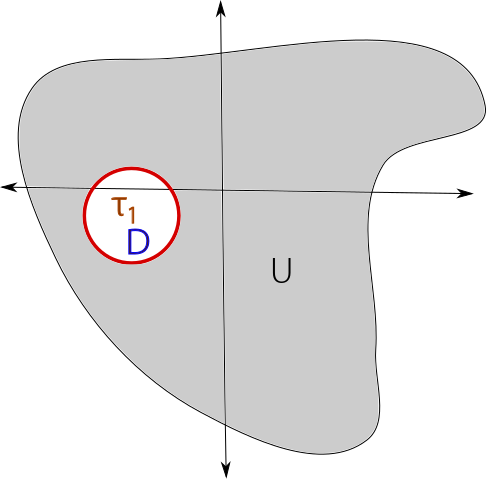
\includegraphics[width=80mm]{drawing86.png}
\end{center}
For the finite rank operator, recall that we have the following definition:
\definition
$F\in \Psi^{-\infty}(Y)$ is of finite rank if there exists $C^{\infty}$ functions $\phi_i, \psi_i$ such that
\begin{align}
F(y,y')=\sum^{N}_{i=1}\phi_{i}(y)\psi_i(y)
\end{align}
\proof
We now begin the length proof. Let $F$ be a finite rank operator such that $|K-F|_{\infty}<\frac{1}{2}$, where $|\cdot |_{\infty}$ is the supreme norm. Then we know that via constructing a Neumann series that 
\begin{align}
I-K(\tau)+F:C^{\infty}(Y)\rightarrow C^{\infty}(Y)
\end{align}
is invertible. We just need to show that for $R=K(\tau_0)-F$, we have $(Id-R)^{-1}=Id+\sum^{\infty}_{j=1}R^{j}$, which converges in the Banach space of operators $C^{0}(Y)\rightarrow C^{0}(Y)$ under $\sup$-norm. We can prove the theorem near a neighborhood of $\tau_1$ and then use elementary complex analysis. 

Moreover, we have $(Id-K(\tau_0)+F)^{-1}=Id-S$, where $S\in \Psi^{-\infty}(Y)$:
\begin{align}
S(y,y')&=\sum^{\infty}_{j=1}R^{j}\\
&=R+R\circ R+R\circ S\circ R\\
&=R(y,y')+\int R(y, z)R(z,y')dz+\int R(y,z)S(z,w)R(w,y')dzdw
\end{align}
We claim that $S(y,y')$ is actually holomorphic in $y,y'$. This follows from (164) since $S(y,y')$ is bounded from (162) with $|R|_{\infty}$ value small enough and each $R^{j}$ is holomorphic. So the limit must be holomorphic. In fact by continuity, there exists $\delta$ such that if $|\tau-\tau_0|\le \delta$, we have 
\begin{align}
R=|K(\tau)-F|_{\infty}<\frac{1}{2\text{Vol}Y^2}
\end{align}
Therefore the above argument shows $(Id-K(\tau)+F)^{-1}$ exists for all $\tau$ with $|\tau-\tau_0|<\delta$. 

A variant of this argument with $S=R+R\circ S$ would not work because we would not be able to use $S$ being bounded to deduce anything about holomorphic. 


We observe that, for any $\tau\in \mathcal{U}$, we have $Id-K(\tau)=Id-K(\tau)+F-F$. We know that for $\tau$ near $\tau_0$, the operator $(Id-K(\tau)+F)^{-1}$ exists. \textbf{We want to write it out explicitly and assert that $(Id-K(\tau))^{-1}$ exists as well. }
\remark
Not really sure how to use it or why this cancellation thing is useful. 

\discussion 
We observe that after cancellation of identical terms we have
\begin{align}
(Id-K(\tau))(Id+S(\tau))&=Id-F\circ (Id+S(\tau))
\end{align}
Since $F$ is a finite rank operator, using Einstein notation we can write
\begin{align}
F(y,y')=\sum \phi_i(y)\circ \psi_i(y')=\phi_i(y) \circ \psi_i(y')
\end{align}
Now for any $\phi\in C^{\infty}(Y)$ we have
\begin{align}
F\circ (Id+S(\tau))\circ \phi&=\int F(y,y')(\phi(y')+S(\tau)\phi(y')dy')\\
&=\phi_i \psi_i(\phi+S\phi)\\
&=\phi_i(\psi_i \phi_i+S^{T}\psi_i)\\
&=\phi_i\xi_i, \xi_i=\psi_i\phi_i+S^{T}\psi_i
\end{align}
Therefore we have
\begin{align}
(Id-K(\tau))(Id+S(\tau))=Id-H(\tau)
\end{align}
where
\begin{align}
H(\tau)=\phi_i(y)\xi_i(\tau,y'), \xi(\tau,y')=\psi_i(y')+S(\tau)^{T}\psi(y')
\end{align}
\remark
The original notes used $F(\tau)$ twice, which I think caused some confusion later in the notation. 
\discussion
Note that for $\tau\in B_{\delta}$ we have $(Id-K(\tau))^{-1}$ exists equivalent to $(Id-H(\tau))^{-1}$ exists because $I+S(\tau)$ is invertible for all $\tau\in B_{\delta}$ via equation (172). So we just need to analyze $(I-H(\tau))^{-1}$. 

Let $\pi$ be orthogonal project onto the space spanned by $\{\overline{\phi}_{i}, i=1\cdots N \}$, where we assume $\phi_i$s are orthonormal via Gram-Schmidt procedure. Then we can write
 \begin{align}
H=\phi_i\cdot (\pi \xi_i)+\phi_i\cdot (Id-\pi)\xi_i
 \end{align}
 where the projection maps $\pi$ are given explicitly by
  \begin{align}
\pi(\xi_i)(\tau,y')&=\langle \xi_i(\tau),\overline{\phi}_{j}\rangle \overline{\phi}_{j}(y')\\
&=(\int \psi_{i}(\tau,y'')\overline{\phi}_{j}(y'')dy'')\overline{\phi}_{j}(y')\\
&=a_{ij}(\tau)\overline{\phi}_{j}(y')
  \end{align}
  where $a_{ij}(\tau)$ is holomorphic for $\tau$ in $B_{\delta}$ since all $\xi_i$ are holomorphic in $\tau$ to begin with. 

Therefore to summarize we have 
  \begin{align}
H(\tau)(y,y')=\phi_i(y)\cdot a_{ij}(\tau)\overline{\phi}_{j}(y')+\phi_i(y)\cdot (Id-\pi)\xi_i
  \end{align}

Now we can decompose $C^{\infty}(Y)$ into $V\oplus V^{\perp}$, with $V$ be the space spanned by $\overline{\phi}_i$. Then under this basis we have $H(\tau)$ to be 
\begin{align}
V\oplus V^{\perp}\rightarrow V\oplus V^{\perp}
\end{align}
and $H(\tau)$ will be of the form
\begin{align}
\begin{bmatrix}
A && B\\
0 && 0
\end{bmatrix}
\end{align}
where $A, B$ is given by:
\begin{align}
A=a_{ij}\langle *,\phi_j\rangle \phi_i+B, B=\phi_i(I-\pi)\xi_i
\end{align}
As a result now we can write $I-H(\tau)$ explicitly as
\begin{align}
\begin{bmatrix}
I-A(\tau) && B(\tau)\\
0 && I
\end{bmatrix}
\end{align}
and it is clear that $I-H(\tau)$'s inverse exists if and only if $I-A(\tau)$'s inverse exists. If this is the case we would have
\begin{align}
(I-H(\tau))^{-1}=
\begin{bmatrix}
[I-A(\tau)]^{-1}&& -[I-A(\tau)]^{-1}B(\tau)\\
0 && I
\end{bmatrix}
\end{align}
Thus we may reduce the invertibility of an operator $I-H(\tau)$ on $C^{\infty}(Y)$ to invertibility of a holomorphic matrix in $\C^{N}$. We know via linear algebra that $I-A(\tau)$'s inverse exists if and only if its determinant is not zero. But $\det(I-A(\tau))$ can only be zero at most $N$ discrete values as it is an algebraic function of $\tau$ determined by $A_{ij}$. Thus $(I-A(\tau))^{-1}$ is a meromorphic function in $\tau$ with poles of order given by the multiplicity of the zeros of its determinant. 

Now let us go back to (172), we can now assert that  $Id-K(\tau)$'s inverse exists except at a discrete set where $\det(I-A(\tau))=0$. Near the discrete set we have $(I+K(\tau))^{-1}=I+M(\tau), M(\tau)\in \Psi^{-\infty}(Y)$, which is given by the explicit formula we had earlier. It is meromorphic and has finite rank singularities. 
\qed 
We thus claim that for $A\in \Psi^{m}_b(X)\in x^{\beta}S(X)$, we have $\widehat{A}(\tau)^{-1}$ to be meromorphic and in the space $\hat{\Psi}^{-m}(Y)$. 

\remark
Do we have to double check the inverse's kernel belong to the space $\mathcal{S}_{ff}^{0}*\Omega_{b, R}$? It seems not really related as $Y$ is compact and all operations can be bounded by a constant. 

\remark
For the last statement, if we are working with normal operators, then should not we working with $\widehat{\Psi}^{m}$ already? Did Prof. Loya forgot the $\widehat{}$ sign?

\section{Lecture 15: Analytical Fredholm theory, Part II}
\definition 
A family $A(\tau)\in \Psi^{m}(Y)$ is holomorphic  for $\tau\in \U$ (where $\U\subset \C$ is open) if 
+
For all locally coordinate patches 
\begin{align}
\phi A(\tau) \psi=\int e^{i(y-y')\cdot \eta}a(\tau, y, \eta)d\eta dy'
\end{align}
where $\phi,\psi$ are compacted supported in coordinate patch, and $a(\tau, y,\eta)$ is holomorphic in $\tau$. 
+
For all $\phi,\psi\in C^{\infty}(Y)$ with disjoint supports, we have
\begin{align}
\phi A \psi=K(\tau, y,y')dy', K\in C^{\infty}(\U\times Y\times Y)
\end{align}
and $K$ is holomorphic in $\tau$. 

\example 
If $A\subset \Psi^{m}_b(X)$ then $\widehat{A}(\tau)$ is a holomorphic family of $\Psi DO$s of order $m$ for $\tau\in \U=\C$. 

\definition 
A holomorphic family $A(\tau)\in \Psi^{m}(Y), \tau\in \U$ is elliptic if there exists a holomorphic family $B(\tau)\in \Psi^{-m}(Y)$ such that $A(\tau)B(\tau)=Id-R(\tau)$. for a holomorphic $R(\tau)\in \Psi^{-\infty}(Y)$. 

\example 
If $A\in \Psi^{m}_b(X), m\in \R$ is elliptic, then there exists $B\in \Psi^{-m}_b(X)$ such that $AB=I-R, R\in \Psi^{-\infty}_{b}(X)$. This implies that
\begin{align}
\widehat{A}(\tau)\circ \widehat{B}(\tau)=I-\widehat{R}(\tau)
\end{align}
and $\widehat{A}(\tau)$ is an elliptic family. 

\example 
Let $\U\subset \C$ be open and connected. Let $K(\tau)\in \Psi^{-\infty}(Y)$ be a holomorphic family. Then $A(\tau)=I-K(\tau)\in \Psi^{0}(Y)$ is an elliptic holomorphic family. Let $B(\tau)=I$. Now trivially we have $AB=I-K(\tau), K(\tau)\in \Psi^{-\infty}(Y)$. If $A(\tau_0)^{-1}$ exists for some $\tau_0\in \U$, then via analytical Fredholm theory we know that $A(\tau)^{-1}=(I-K(\tau))^{-1}$ is meromorphic with values in $\Psi^{0}(Y)=I+\Psi^{-\infty}(Y)$. In other words it has at most finite rank singularities. 

\theorem 
There is an analytical Fredholm theory for general elliptic families. Let $\U\subset \C$ be open and connected. Let $A(\tau)\in \Psi^{m}(Y)$ be a holomorphic elliptic family. Also assume that there exists $\tau_0\in \U$ such that $A(\tau_0)^{-1}$ exists. 

Then the corresponding analytical Fredholm theory asserts that $A(\tau)^{-1}$ is a meromorphic family of operators in $\Psi^{-m}(Y)$ having finite rank singularities. In other words, there exists a finite discrete set $D$ such that for $\U/D$, the operator $A(\tau)^{-1}$ exists and is a holomorphic family $A(\tau)^{-1}\in \Psi^{-m}(Y)$. 

Near points in $D$, we claim that $A(\tau)^{-1}$ can be expressed as follows: If $\tau_1\in D$, then there exists open disk $B\subset \U$ centered at $\tau_1$ such that 
\begin{align}
A(\tau)^{-1}=B(\tau)+\sum \frac{F_k}{(\tau-\tau_1)^{k}}, k=1\cdots N
\end{align}
where $B(\tau)\in \Psi^{-m}(Y)$ is a holomorphic family such that $F_{i}$ are finitely many finite rank operators. 

\comment 
This is the operator version of $f:\U\rightarrow \C$ being holomorphic, then near the zero of $f$ we have
\begin{align}
\frac{1}{f(\tau)}=\sum_{k}\frac{1}{(\tau-\tau_i)^{k}}
\end{align}
\proof
By definition of elliptic family, there exists $P(\tau)\in \Psi^{-\infty}(Y)$ such that $A(\tau)P(\tau)=I-K(\tau)$, where $K(\tau)\in \Psi^{-\infty}(Y)$ is a holomorphic family. We can approximate $K(\tau_0)$ be a finite rank operator such that $(I-K(\tau_0)+F)$ is invertible. 

We now observe that 
\begin{align}
A(\tau)(P(\tau)+A(\tau_0)^{-1}K(\tau))=I-K(\tau)+A(\tau)A(\tau_0)^{-1}K(\tau)
\end{align}
If we let the term on the right to be
\begin{align}
\tilde{K}(\tau)=A(\tau)A(\tau_0)^{-1}K(\tau)-K(\tau)
\end{align}
as well as
\begin{align}
\tilde{P}(\tau)=P(\tau)+A(\tau_0)^{-1}K(\tau)
\end{align}
then we can simply re-write equation (189) as 
\begin{equation}
A(\tau)\tilde{P}(\tau)=I-\tilde{K}(\tau),  \tilde{K}(\tau_0)=0
\end{equation}
Therefore trivially we have $(I-\tilde{K}(\tau_0))^{-1}=I$ exists. Now the original analytical Fredholm theory says that $I-\tilde{K}(\tau)$'s inverse would be exist and equal to $I+R(\tau)\in \Psi^{-\infty}(Y)$, which is meromorphic with finite rank singularities. As a result we have
\begin{align}
A(\tau)^{-1}&=\tilde{P}(\tau)(I-\tilde{K}(\tau))^{-1}\\
&=\tilde{P}(\tau)+\tilde{P}(\tau)\circ R(\tau)
\end{align}
It is now easy to check that $\tilde{P}(\tau)\circ R(\tau)\in \Psi^{-\infty}(Y)$ is meromorphic with values in $\Psi^{-\infty}(Y)$ with finite rank singularities. 
\qed
\remark
In the original notes it says $K(\tau)$ instead of $R(\tau)$, which does not make sense to me. 
\subsection{Exercise for Lecture 14} 
\exercise 
Let $m>0$, let $A\in \Psi^{m}(Y)$ be elliptic. 
+
Prove that $A(\tau)=A-\tau$ is an elliptic family of holomorphic operators for $\tau\in \C$. 

By analytical Fredholm theory, if there exists $\tau_0\in \C$ such that $(A-\tau_0)^{-1}$ exists, then $(A-\tau)^{-1}$ which is the resolvent of $A$ is meromorphic with values in $\Psi^{-m}(Y)$ with finite rank singularities. 
\proof
Clearly if $A$ is elliptic, then $cA$ is elliptic for $c\not=0$. So it suffice to assume $\tau=1$ since $\tau=0$ case is solved by the hypothesis. Now let $B\in \Psi^{-m}$ the paramatrix from the small-calculus:
\begin{align}
AB=I-R
\end{align}
Now formally we have
\begin{align}
(A+I)B=AB+B=I+(B-R)
\end{align}
we can now multiply a Newmann series on both sides to cancel out the $I+(B-R)$ factor up to an $\Psi^{-\infty}$ term. Now we have
\begin{align}
(A+I)B(I+S)=I+R_2
\end{align}
Therefore $A+I$ is elliptic with a paramatrix equal to $B(I+S)$. 
\qed 
+
Assume now that $A\in \Psi^{m}(Y)$ is self-adjoint: $\langle A\phi, \psi\rangle=\langle \phi, A\psi\rangle$ for all $\phi, \psi\in C^{\infty}(Y)$. Prove that for all $\tau_0$ with non-zero imaginary part, the operator $A-\tau_0$ is invertible. 
\proof
Assume $A-\tau_0$ is not invertible for some $\tau_0$ with non-zero imaginary part.We can absorb the real part into $A$, and up to rescaling of the imaginary part we may assuming $\tau=i$.  Thus there exists some $v\not=0$ such that
\begin{align}
\langle Av, v\rangle=\langle iv, v\rangle=i\langle v, v\rangle=\langle v, -iv\rangle=\langle v, Av\rangle 
\end{align}
where the last arrow follows from self-adjointness of $A$ and the middle from the conjugate linear definition of the inner product. But $Av=iv=-iv$ is absurd unless $v=0$. Therefore $A-\tau_0$ must be invertible as desired. 

\qed
+
If $A$ is self-adjoint as above, prove that 

1) $(A-\tau)^{-1}$ only fails to exist in a discrete subset of $D$ of real number.
\proof
Suppose that $(A-\tau)^{-1}$ fails to exist, then the above argument showed $\tau$ must be real. Now if $(A-\tau)^{-1}$ fails to exist on an infinite sequence of points
\begin{align}
\tau_{n}\rightarrow \tau', \tau'\in \C
\end{align}
Then $A-\tau$ must be zero operator from elementary complex analysis, as the zeros of a holomorphic operator are isolated judged from local Taylor series expansion. But our hypothesis is that $(A-\tau_0)^{-1}$ exists at some point, contrary to this result. Therefore $(A-\tau)^{-1}$ only fails to exist in a discrete subset $D$ of real number. 
\qed

2) $(A-\tau)^{-1}$ has at most simple poles. In other words, if $\tau_1\in D$, then near $\tau_1$ we have
\begin{align}
(A-\tau)^{-1}=B(\tau)-\frac{F}{\tau-\tau_1}
\end{align}
where $F$ is finite-rank and $B(\tau)$ is in $\Psi^{-\infty}(Y)$ which is holomorphic in $\tau$. 
\proof
We try to use the comment 2 below. We want to show that
\begin{align}
|\langle (A-iy)^{-1}\phi, \phi\rangle|\le C\frac{1}{|y|}\langle \phi, \phi\rangle 
\end{align}
Let $\phi=(A-iy)\psi$. Then we have (202) is equivalent to
\begin{align}
|\langle \psi, (A-iy)\psi\rangle|\le C\frac{1}{|y|}\langle (A-iy)\psi, (A-iy)\psi\rangle
\end{align}
Expand out the right hand side we get
\begin{align}
\langle (A-iy)\psi, (A-iy)\psi\rangle=\langle A\phi, A\phi\rangle+\langle -iy\psi, -iy\psi\rangle+\langle A\psi, -iy\psi\rangle+\langle -iy\psi, A\psi\rangle
\end{align}
But by the fact that $\langle av, bu\rangle= a\overline{b}\langle v,u\rangle$ and $A$ is self-adjoint, we have
\begin{align}
\langle -iy\psi, A\psi\rangle=-iy\langle \psi, A\psi\rangle=-iy\langle A\psi, \psi\rangle, \langle A\psi, -iy\psi\rangle=iy\langle A\psi, \psi\rangle
\end{align}
as well as
\begin{align}
\langle -iy\psi, -iy\psi\rangle=-iy\langle \psi, -iy\psi\rangle=y^{2}\langle \psi, \psi\rangle
\end{align}
Therefore after some cancelling we have to show that
\begin{align}
|\langle \psi, (A-iy)\psi\rangle|\le C\frac{1}{|y|}(\langle A\psi, A\psi\rangle+y^2\langle \psi, \psi\rangle)=C\frac{1}{|y|}\langle A\psi, A\psi\rangle +C|y|\langle \psi, \psi\rangle
\end{align}
Using triangular inequality we trivially have
\begin{align}
|\langle \psi, (A-iy)\psi\rangle|\le |\langle \psi, A\psi\rangle|+|y|\langle \psi, \psi|\rangle
\end{align}
Hence it only remains to show that there exist some $C$ such that
\begin{align}
\langle \psi, A\psi\rangle\le C\frac{1}{|y|}\langle A\psi, A\psi\rangle
\end{align}
\remark 
At this step I got stuck. Perhaps my approach does not work?
\qed
\\
3) Moreover, we have explicit formula for $F$ and $B$:
\begin{align}
F=\Pi_{\ker(A-\tau_1)}, B(\tau_1)=
\begin{cases}
0& \text{On  } \ker(A-\tau_1)\\
 (A-\tau_{1})^{-1} & \text{On  } \ker (A-\tau_1)^{-1}
\end{cases}
\end{align}
In other words $F$ is the orthogonal projection onto the $\tau_1$ eigenvalue of $A$. 
\proof

\qed

\comment 
Prof. Loya provided the following hint. For part (2), for $y\in \R-\{0\}$ and $\phi\in C^{\infty}(Y)$, prove that
\begin{align}
|\langle (A-iy)^{-1}\phi,\phi\rangle|\le C\frac{1}{|y|}\langle \phi,\phi\rangle 
\end{align}

\comment
For part (3), Prof. Loya provided the following hint:
\begin{align}
\textrm{Im}\langle (A-iy)\phi, \phi\rangle=-y\langle \phi, \phi\rangle 
\end{align}

\subsection{Application to the normal operator}
What we did earlier give rise directly to the following theorem: 
\theorem 
Let $A\in \Psi^{m}_{b}(X), m\in \R$ be elliptic. Assume $\widehat{A}(\tau)^{-1}$ exists for all $\tau \in \R$, then there exists $\alpha>0$ such that $\widehat{A}(\tau)^{-1}\in \widehat{\Psi}^{-m,\alpha}(Y)$. 

In other words, there exists $\alpha>0$ such that $\widehat{A}(\tau)^{-1}$ exists on the strip $\Omega_{\alpha}$. Further $\widehat{A}(\tau)^{-1}$ must satisfy the following normal operator estimates:
+
If $\phi$ is compactedly supported in a coordinate patch, then
\begin{align}
\phi \widehat{A}(\tau)^{-1}\phi=\int e^{i(y-y')\cdot \eta}a(y,\tau, \eta)d\eta dy'
\end{align}
where $a$ is holomorphic in $\tau\in \Omega_{\alpha}$ and 
\begin{align}
|\partial^{\beta}_{y}(\partial_{\tau}\partial_{\eta})^{\alpha}a(y,\tau, \eta)|\le (1+|\eta|+|\tau|)^{-m-|\alpha|}
\end{align}
\remark
Prof. Loya wrote $-m-|\gamma|$, which does not make sense to me as $|\gamma|$ did not even show up on the left hand side. 

+
If $\phi, \psi\in C^{\infty}(Y)$ have disjoint supports, then we have $\phi\widehat{A}(\tau)\psi\in \Psi^{-\infty,\alpha}(Y)$. 

\comment Here is a graph of $\Omega_{\alpha}$:
\begin{center}
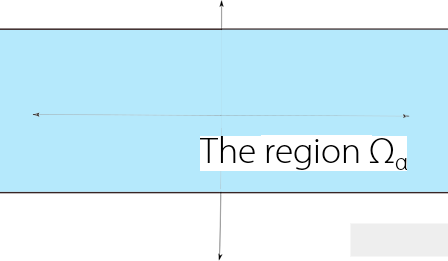
\includegraphics[width=100mm]{drawing92.png}
\end{center}

\proof
Since $A$ is elliptic, by definition we know there exists $B\in \Psi^{-m}_b(X)$ such that $AB=I-R$, where $R\in \Psi^{-\infty}_b(X)$ is smoothing. Thus we have $\widehat{A}(\tau)\widehat{B}(\tau)=I-\widehat{R}(\tau)$. Now we know $\widehat{R}(\tau)\in \widehat{\Psi}^{-\infty}(Y)$. Therefore $\widehat{R}$ is smoothing and its kernel can be written as
\begin{align}
\widehat{R}(\tau, y, y')\in C^{\infty}(\C\times Y\times Y)
\end{align}
and it is Schwartz in $\tau$ for $\tau \in \Omega_1$ since it is holomorphic in the first coordinate. See Example 8, Definition 11 and Lecture 13. 

In other words, for any $k\in \N$ and $P, P'\in \textrm{Diff}^{*}(Y)$ and $l\in \N$ we have
\begin{align}
|\partial^{k}_{\tau}P_{y}P'_{y'}R(\tau, y, y')|\le C_{l, k}(1+|\tau|)^{-l}
\end{align} 

Therefore there exists some $a_1$ such that
\begin{align}
(I-\widehat{R}(\tau))^{-1}
\end{align}
exists for all $\tau\in \Omega_1$ with $|\Re \tau|\ge a_1$. See the attached picture:
\begin{center}
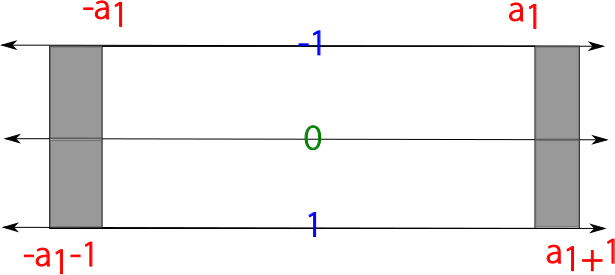
\includegraphics[width=100mm]{drawing93.png}
\end{center}
Hence we know that $\widehat{A}(\tau)\widehat{B}(\tau)(I-\widehat{R}(\tau))^{-1}=Id$ exists for $\tau\in \Omega$, and $|\Re \tau|\ge a_1$. Hence $\widehat{A}(\tau)^{-1}$ exists for all $\tau\in \Omega_1$, $|\Re \tau|\ge a_1$. Otherwise we would have a contradiction as right hand side is $Id$.  Also we note that $\widehat{A}(\tau)$ is a holomorpic family of operators on the region $\U=\{\tau\in \Omega_1, |\Re \tau|<a_1+1\}$. 
\remark
Unclear to me why this is needed: Is this because of the choice of $D$ or something?
\discussion 
Therefore $\hat{A}(\tau)^{-1}$ exists for all $\tau\in \U$ with $a_1\le |\Re \tau|<a_1+1$:
\begin{center}
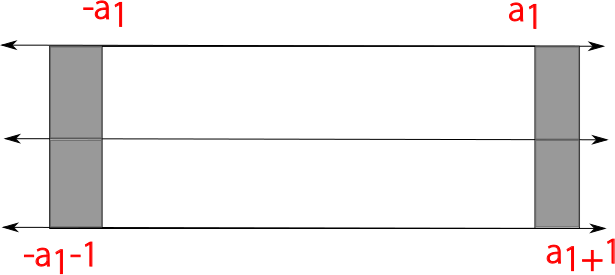
\includegraphics[width=100mm]{drawing94.png}
\end{center}
see the above picture. The analytical Fredholm theory says that $\widehat{A}(\tau)^{-1}$ exists for all $\tau \U$ except at some discrete set $D$:
\begin{center}
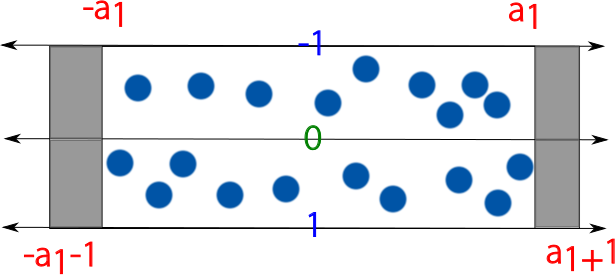
\includegraphics[width=100mm]{drawing95.png}
\end{center}
where there are no poles on the real line because by assumption $\widehat{A}(\tau)$ exists for all $\tau\in \R$. Now by elementary complex analysis we assert that there exist $\alpha$ such that $\hat{A}(\tau)^{-1}$ exists for all $\tau\in \U$ with $|\Im \tau|\le \alpha$:
\begin{center}
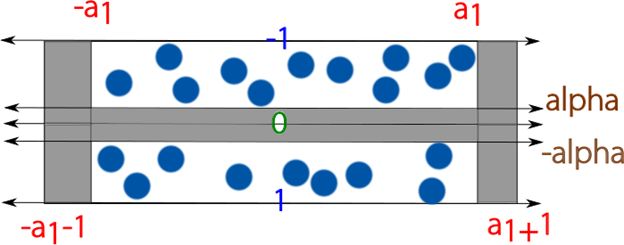
\includegraphics[width=100mm]{drawing96.png}
\end{center}
Therefore if we choose $\Omega_{\alpha}$ according to this $\alpha$, then we are done! The formula for its inverse would be 
\begin{align}
\widehat{A}(\tau)^{-1}=\widehat{B}(\tau)(I-\hat{R}(\tau))^{-1}
\end{align}
\remark
I suspect there is a typo here in the original notes, which claim the second term is $(I-\widehat{B}(\tau))$, which does not make sense. 
\discussion 
It now only remain to verify the symbol estimates. We still have to show that $\hat{A}(\tau)^{-1}\in \Psi^{-m}(Y), \tau\in \Omega_{\alpha}$. We can actually show something stronger: $\widehat{A}(\tau)^{-1}\in \widehat{\Psi}^{-m,\alpha}(Y)$. 

\exercise 
Prove this using the fact that we know for $\tau\in \Omega_1$, $|\Re \tau|\ge a_1$, we have $(I-R(\tau))^{-1}=I+S(\tau)$, where $S(\tau)\in \Psi^{-\infty}(Y)$ is a holomorphic family for $\tau\in \Omega_1$ with $|\Re \tau|\ge \alpha_1$. 

\comment Hint: Use that
\begin{align}
A(\tau)^{-1}=\widehat{B}(\tau)+\widehat{B}(\tau)S(\tau), \tau\in \Omega_{\alpha}, |\Re(\tau)|\ge a_{1}
\end{align}
to get estimate for $S(\tau)$ needed to show that $\widehat{A}(\tau)^{-1}\in \widehat{\Psi}^{-m,\alpha}(Y)$. 
\qed 

\section{Lecture 16: Fredholmness in the space $x^{\epsilon}\mathcal{S}^{0}$}
\subsection {interlude}
Adam started a question on the operator $x\partial_{x}$, which he claim to be equal to $\int e^{iz\cdot \tau}i\tau d\tau$. The surprisingly discovery is that it is zero off the diagonal as a distribution. Prof. Loya showed this during the beginning and end of the class. 

\subsection{class discussion}
We had just proved this theorem:
\theorem 
If $A\in \Psi^{m}_b(X)$ and $\widehat{A}(\tau)^{-1}$ exists for all $\tau\in \R$, then there exists $a>0$ such that $\widehat{A}(\tau)^{-1}\in \widehat{\Psi}^{-m,\alpha}(Y)$. Therefore $\widehat{A}(\tau)$ is Fredholm. Now recall if $A\in \Psi^{m,\alpha}_b(X)$, then for all $\beta \in \R$, $|\beta|<\alpha$, we have $A:X^{\beta}S^{0}(X)\rightarrow X^{\beta}S^{0}(X)$ is continuous. 

\lemma
Let $R\in S^{0}(X^2)$, let $\epsilon>0$, then let $S=x^{\epsilon}(x')^{\epsilon}Ru'$, with $u\in C^{\infty}(X,\Omega_b)$. Then we claim that $S$ is in the space $P^{\epsilon}_{lb}P^{\epsilon}_{rb}P^{2\epsilon}_{\textrm{front face}}S^{0}$.  

We have the following picture:
\begin{center}
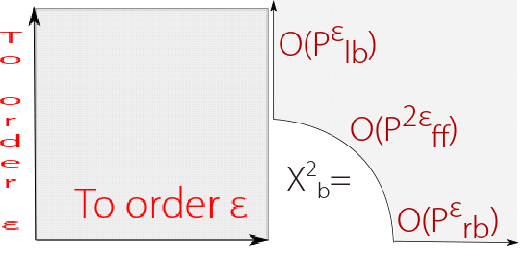
\includegraphics[width=100mm]{drawing97.png}
\end{center}
\proof
Prof.Loya claimed that the proof is "easy".  To show it we divide into two cases as before:
\begin{center}
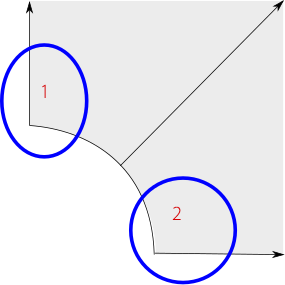
\includegraphics[width=60mm]{drawing88.png}
\end{center}
In the first coordinate we have $z_1=\frac{x}{x'}, z_2=x'$. In the second coordinate we have $z_1=x, z_2=\frac{x'}{x}$. 

Observe that off the front-face we have $S^{0}(X^2)=S^{0}(X^2_b)$. This Prof. Loya claimed to be trivial because we are using $b$-derivatives. And $b$-derivatives in the projective coordinates are the same as in ordinary coordinates. 

In the neighborhood (1) we have $x=rw, x'=r$, which implies that
\begin{align}
x^{\epsilon}x'^{\epsilon}&=(rw)^{\epsilon}r^{\epsilon}\\
&=r^{2\epsilon}\cdot w^{\epsilon}\\
&=P^{2\epsilon}_{ff}\cdot P^{\epsilon}_{lb}
\end{align}
and in the second neighborhood (2) we have $x=r, x'=rw$, with implies that
\begin{align}
x^{\epsilon}x'^{\epsilon}&=r^{2\epsilon}w^{\epsilon}\\
&=r^{2\epsilon}w^{\epsilon}\\
&=P^{2\epsilon}_{ff}P^{\epsilon}_{rb}
\end{align}
\qed 
\comment
Prof. Loya comment that $\epsilon$-decay corresponding to exponential decay on the cylinder. 

\remark 
If $K\in x^{\epsilon}x'^{\epsilon}S^{0}(X^2)$, then for any $b$-density $\mu$, the operator
\begin{align}
K=u\mu', K\phi=\int u(x',x)\phi(x')\mu(x')
\end{align}
is a ``true residual" operator in the sense that it is the limit of finite rank operators on $X^{\beta}C^{0}(X)$ for any $\beta\in \R$ with $|\beta|<\epsilon$. Note here that by choosing $C^{0}(X)$ instead of $S^{0}(X)$, we are actually working with a Banach space instead of a locally Frechet space, in which the limit of finite rank operators is a true compact operator. 

Here is our main theorem for this lecture: 
\theorem 
Let $A\in \Psi^{-m}_b(X)$ be elliptic, and assume that $\widehat{(\tau)}^{-1}$ exists for all $\tau\in \R$. Then for all $\beta$ in $\R$ with $|\beta|$ sufficiently small, we claim that $A:X^{\beta}S^0(X)\rightarrow X^{\beta}S^0(X)$ is Fredholm. 
\proof
The strategy is now familiar. We know that $\hat{A}(\tau)^{-1}\in \widehat{\Psi}^{-m,\alpha'}(Y)$. Let $B_0\in \Psi^{m,\alpha}_b(X)$ with $\alpha<\alpha'$ such that $\widehat{B}_0(\tau)=\widehat{A}(\tau)^{-1}$. Recall that we can just take
\begin{align}
B_0=\phi \int e^{iz\cdot \tau}\widehat{A}(\tau)^{-1}d\tau
\end{align}
\begin{center}
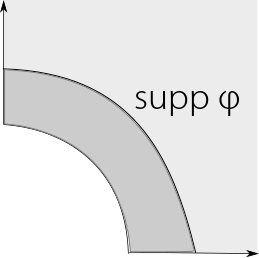
\includegraphics[width=60mm]{drawing98.png}
\end{center}
Now as usual we can take a small paramatrix: We have 
\begin{align}
AB_1=Id-R_1, B_1\in \Psi^{-m}_{b}(X), R\in \Psi^{-\infty}_{b}(X)
\end{align}
Now if we let $B_2=B_1+B_0\circ R_1$, then we have
\begin{align}
A\circ B_2=Id-R_2, R_2\in \Psi^{-\infty, \alpha}_b(X), \widehat{R}_2(\tau)=0
\end{align}
this implies that $R_2\equiv 0$ on the front face. 

We recall that if we let $\alpha_0=\min(1,\alpha)$, then we have the following picture:
\begin{center}
	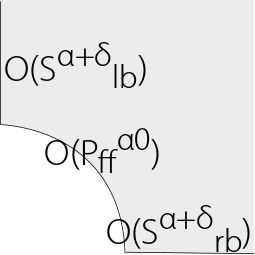
\includegraphics[width=60mm]{drawing99.png}
\end{center}
Recall that we have $R(r,z)=R_0(z)+r^{\alpha_0}(r,z)=O(1)+r^{\alpha_0}R_1(r,z)\in \mathcal{S}^{0}$. Therefore if we let $\epsilon=\frac{\alpha_0}{2}$, then $R_0\in P^{\epsilon}_{lb}P^{\epsilon}_{rb}P^{2\epsilon}_{\textrm{front face}}\mathcal{S}^{0}(X^2_b)$. Now by the lemma we have 	$R_2\in x^{\epsilon}x'^{\epsilon}S^{0}X^2$. Now by the Stone-Weistrauss theorem, we claim that the subspace generated by operators of the form $x^{\epsilon}S^{0}(X)\otimes x'^{\epsilon}S^{0}(X)$ is dense in the sup-norm in the space of continuous functions that vanishes at $\partial (X^2)$. In other words, for all $\mu\in C^{0}(X^2)$, there exist $\mu_{i}\rightarrow \mu$ in $C^{0}(X)\times C^{0}(X)|_{\sup}$. In particular there exist $F=\sum \phi_i(x)\otimes \psi_i(x')$, with $\phi_i \in x^{\epsilon}S^{0}(X), \psi_i\in  x;^{\epsilon}S^{0}(X)$, such that $|R_2-F|_{\infty}\le \frac{1}{2 \text{Vol}(Y\times Y)}$. 

Now we may carry out the same program as last time: We have
\begin{align}
A\circ B_2=I+R_2-F+F
\end{align}
and 
\begin{align}
S=\sum^{\infty}_{k=1}(-1)^{k}(R_2-F)^{k}, R_2'=F-R_2
\end{align}
and we know that $S\in C^{0}(X)$ because $S=R_2'+R_2'\circ R_2'+R'_2\circ S\circ R_2'\in x^{\epsilon}x'^{\epsilon}\mathcal{S}^{0}(X^2)$. The $x^{\epsilon}x'^{\epsilon}$ factor corresponds to exponential decay, which guarantees $R_2'$ to be integrable in both variables in the middle. As a result we conclude that $S\in x^{\epsilon}x'^{\epsilon}\mathcal{S}^{0}(X^2)$ as well. Moreover we have the following identity:
\begin{align}
S&=R_2'+R_2\circ S\\
&-R_2'+S\circ R_2'
\end{align}
Therefore we now have 
\begin{align}
A\circ B_2(Id+S)&=(I-R_2)(I+S)+F(I+S)\\
&=I-R_2'+S-R_2'\circ S+F(I+S)\\
&=I+F(I+S), F\in x^{\epsilon}(\mathcal{S}^{0}X)x'^{\epsilon}(\mathcal{S}^{0}X) \textrm{ is finite rank}
\end{align}
Let $B=B_2+B_2\circ S, F=F\circ (I+S)$. We have $B\in \Psi^{-m,\alpha}, S\in x^{\epsilon}x'^{\epsilon}\mathcal{S}^{0}(X^2)=P^{\epsilon}_{lb}P^{\epsilon}_{rb}P^{2\epsilon}_{\textrm{front face}}\mathcal{S}^{0}(X^2_b)\subseteq \Psi^{-\infty, \epsilon'}_{b}(X), \epsilon'=\frac{\epsilon}{2}$, $B_2\in \Psi^{-m,\alpha}_{b}(X)\subset \Psi^{-m,\epsilon'}_{b}(X), \epsilon'<\alpha$. 

Finally we have $A\circ B=I+F', B\in B\in \Psi^{-m,\epsilon'}(X),\epsilon'>0$, $F'\in x^{\epsilon}(\mathcal{S}^{0}X)x'^{\epsilon}(\mathcal{S}^{0}X)$ and is finite rank as required. This finished the proof. We only need to choose $\beta\in \R$ with $|\beta|<\epsilon'$, then $A\circ B=I+F'$:
\begin{align}
X^{\beta}S^{0}(X)\rightarrow X^{\beta}S^{0}(X)
\end{align}
as well as $F'$ is finite rank. So $A$ is Fredholm. 
\qed

\example 
Let us talk about the Dirac operator. Let 
\begin{align}
D:C^{\infty}(X,E)\rightarrow C^{\infty}(X,E)
\end{align}
with $D$ a first-order differential operator such that on a collar of $X\cong [0,1]_X\cong Y$:
\begin{center}
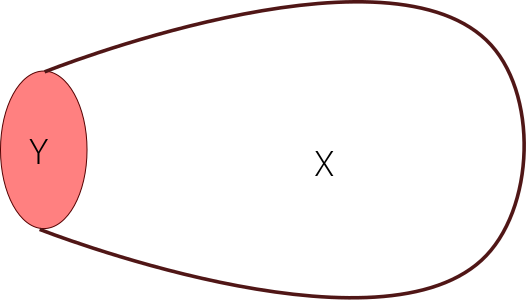
\includegraphics[width=100mm]{drawing83.png}
\end{center}
we have
\begin{align}
D=\frac{1}{i}\sigma(x\partial_{x}+D_y)
\end{align}
where $\sigma$ is in $C^{\infty}(X, Hom(E))$, and $D_{y}:C^{\infty}(Y, E_{0})\rightarrow C^{\infty}(Y, E_0)$ is self-adjoint. Here $E_0=E|_{\partial_{X}}$. This will be the model case we are interested. 

\theorem 
We have $\widehat{D}(\tau)^{-1}$ exists for all $\tau\in \R$ if and only if $D_0:C^{\infty}(Y,E_0)\rightarrow C^{\infty}(Y,E_0)$ is invertible. 
\proof
We have 
\begin{align}
\widehat{D}(\tau)=\frac{1}{i}(i\tau+D_{y})
\end{align}
Now let $\phi\in C^{\infty}(Y, E_0)$ extend to $\tilde{\phi}\in C^{\infty}(X,E)$. By Lecture 11 and Lecture 12 we should have
\begin{align}
\widehat{D}(\tau)\phi&=x^{-i\tau}Dx^{i\tau}\tilde{\phi}|_{x=0}\\
&=x^{-i\tau}\frac{1}{i}\sigma(i\tau x^{i\tau}\tilde{\phi})+D_0 x^{i\tau}\tilde{\phi}+x^{i\tau}x\partial_{x}\tilde{\phi}|_{x=0}\\
&=\frac{1}{i}\sigma(i \tau \phi+D_0 \phi)
\end{align}
Now as we know $\sigma$ is invertible, and therefore $\widehat{D}(\tau)^{-1}$ exists. But by above computation this holds if and only if $(i\tau+D_0)^{-1}$ exists. We recall that $D_0$ is self-adjoint, so $(i\tau+D_0)^{-1}$ must exist for all $\tau\in \R/\{0\}$ by homework. By assumption $\widehat{D}(\tau)^{-1}$ exist would imply $(i\tau+D_0)^{-1}$ exist for $\tau=0$ as well. Thus $D_0^{-1}$ exists! The logic clearly can go reverse as each step is if and only if. So we finished the proof. 
\qed
\discussion What if it does not exist? 
\theorem 
A generalized Dirac operator is Fredholm via discussion in the following cases. If $D_0$ is invertible, therefore for all $\beta\in \R$ sufficiently small we have
\begin{align}
D:x^{\beta}S^{0}(X,E)\rightarrow x^{\beta}S^{0}(X,E)
\end{align}
then by Theorem 19 we claim $D$ is Fredholm. However, if $D$ is not invertible, then for $|\beta|$ sufficiently small not equal to $0$, we $\textbf{still}$ have $D$ to be Fredholm! 

\proof
This proof is classical and can be quite instructive. Let us consider the operator
\begin{align}
A_{\beta}=x^{-\beta}Dx^{\beta}
\end{align}
on the collar, now via computation we have
\begin{align}
A_{\beta}=\frac{1}{i}(i\tau+\beta+D_0)
\end{align}
then by the previous argument we know that
$\widehat{A}_{\beta}(\tau)^{-1}$ exists for all $\tau\in \R$ if and only if $(\beta+D_0)^{-1}$ exists. We know that this must be true for $|\beta|$ small enough except $|\beta|=0$. We can see this via a plot of $D_0$'s spectrum:
\begin{center}
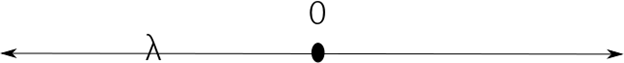
\includegraphics[width=100mm]{drawing100.png}
\end{center}
If $D_)$ is not invertible, then $0$ could be an eigenvalue. However if we shift by $|\beta|<|\lambda|$ with $|\lambda|$ the smallest absolute eigenvalue value, then we claim that $\beta+D_0$ is invertible! Clearly it cannot have an eigenvalue $0$ any more! Now Theorem 19 applies to $A_{\beta}$ and we conclude it is Fredholm $S^{0}(X,E)\rightarrow S^{0}(X,E)$. To finish the proof for $D$ we may want to separate into two cases $0<\beta<\min(\lambda_i)$ and $-\min(|\lambda_i|)<\beta<0$. Therefore we conclude that \begin{align}
D:x^{\beta}S^{0}(X,E)\rightarrow x^{\beta}S^{0}(X,E)
\end{align}
is Fredholm. 

\exercise 
We have two cases, either $\beta>0$ or $\beta<0$. We claim in both cases one has the same index. 

 \section{Lecture 17: Revisit the ${}^{b}$-trace}
This lecture is entirely based on Kunal's notes as I was mostly absent.
\subsection{Adjoints}
Here review the definition of adjoints. Recall that the inner product is defined by
\begin{align}
\langle \phi, \psi\rangle=\int \phi \overline{\psi}\mu
\end{align}
where $\mu$ is a $b$-density. We can also work with real inner products. Now we have
\begin{align}
\langle A\phi, \psi\rangle'=\langle \phi, \overline{A^{T}}\psi\rangle', \phi, \psi\in x^{\epsilon}\mathcal{S}^{0}(X)
\end{align}
If $A\in \Psi^{m,\alpha}_{b}(X)$, then we should have $\overline{A^{T}}\in \Psi^{m,\alpha}_{b}(X)$ as well. We can write $\langle A\phi, \psi\rangle'=\langle \phi, \overline{A^{T}}\psi\rangle'$ as 
\begin{align}
\int (A\phi)(x)\overline{\psi}(x)\mu=\int \phi(x)\overline{\overline{A^{T}}\psi(x)}\mu
\end{align}
To prove that $\overline{A^{T}}\in \Psi^{m,\alpha}_{b}$ as claimed, we will rewrite it in a more useful way. Recall that the inner product is really
\begin{align}
\int (A\phi)(x)\psi(x)\mu=\int \phi(x)A^{T}\psi(x)\mu
\end{align}
and we can rewrite it as
\begin{align}
\int A_{1}K(x,x)\mu=\int A_{2}^{T}K(x,x)\mu
\end{align}
where we define $K(x,x')=\phi(x)\psi(x')\in x^{\epsilon}(\mathcal{S}^{0}X)x'^{\epsilon}(\mathcal{S}^{0}X)$ and $A_1 K$ acting on $x\rightarrow k(x,x')$, $A_2 K=A^{T}$ acting on $x'\rightarrow k(x,x')$. 
\remark
I think some elaboration is needed. 

\exercise 
We have the following theorem:
\theorem 
If $A\in \Psi^{m,\alpha}_{b}(X)$, then there exists $B\in \Psi^{m,\alpha}_{b}(X)$ such that for all $K\in x^{\epsilon}x'^{\epsilon}(\mathcal{S}^{0}[X\times X]$ and $\epsilon>0$, we have
\begin{align}
\int (A_1 K)(x,x)\mu(x)=\int (B_2 K)(x, x)\mu(x)
\end{align}
\comment
The hint is to first prove (243) using partition of unity for $A$, then interpret $B$ as $B(x,x')=A(x',x)$, and $B=A^T$.
\remark
I feel the way Prof. Loya frame everything is still kind of confusing. 
\subsection{${}^{b}$-integral and ${}^{b}$ trace}
Let $A\in \Psi^{-\infty,\alpha}_{b}(X)$, then we have $A(r,z)=\mu_0(z)+r^{\alpha_{0}}\mu_1(r,z),\mu_1\in \mathcal{S}^{0, \alpha_0},\alpha_0=\min\{\alpha,1\}$:
\begin{center}
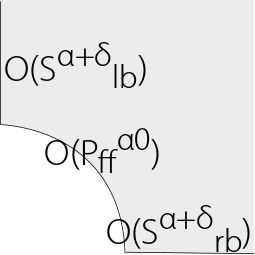
\includegraphics[width=60mm]{drawing99.png}
\end{center}
Therefore we can interpret $A|_{\Delta_b}$ as in the space $\mathcal{S}^{0, \alpha_0}(X, \Omega_b)$. Now we have
\begin{center}
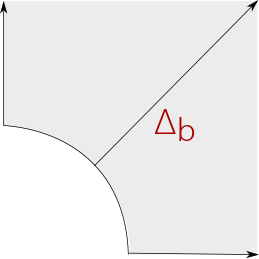
\includegraphics[width=60mm]{drawing101.png}
\end{center}
\begin{align}
A|_{\Delta_b}&=\mu_0(0)+\gamma^{\alpha_0}v_1(r,0)\\&=(v_0(y)+x^{\alpha_0}v_1(x,y))\mu, v_0(y)\in C^{\infty}(Y), v_1(x,y)\in \mathcal{S}^{0},\mu\in C^{\infty}(X, \Omega_b)
\end{align}
\comment
There are in fact $y,y'$ in the above formula. We can in fact re-write the above formula as
\begin{align}
A(r,z,y,y')=\mu_0(z,y,y')+r^{\alpha_0}\mu_1(r,z,y,y')
\end{align}
similarly as $z=0$ on the diagonal we have
\begin{align}
A|_{\Delta_b}=v_0(0,y,y')+r^{\alpha_0}v_1(r, 0, y,y')
\end{align}

\discussion
Our goal for now is to show that $\int A|_{\Delta_b}$ can be interpreted as the trace of $A$ as an operator in some appropriate sense. To do that let us define the integral of densities in $\mathcal{S}^{0,\alpha}(X,\Omega_b)$ first. 

We claim that there are two ways: 
+
This is the first method. Let $\mu\in S^{0,\alpha}(X,\Omega_b)$. We know that $\mu$ restricted to the collar $C=[0,1)_{X}\times Y$
\begin{center}
	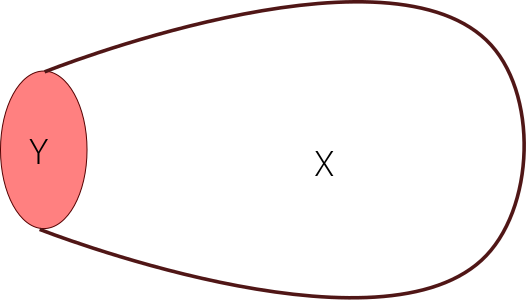
\includegraphics[width=100mm]{drawing83.png}
\end{center}
is of the form
\begin{align}
\mu=\mu_0(y)\frac{dx}{x}dy+x^{\alpha}\mu_1(x,y)\frac{dx}{x}dy
\end{align}
Now the issue is we know
\begin{align}
\int^{1}_{0}\int_{Y}\mu_0(Y)\frac{dx}{x}dy
\end{align}
does not exist because $\int^{1}_{0}\frac{dx}{x}=\infty$. SO we have to get rid of this obstruction. 
\definition 
The ${}^{b}$-integral is defined as
\begin{align}
{}^{b}\int \mu=\int_{X/C}\mu+\int^{1}_{0}\int_{Y}x^{\alpha}\mu_1(x,y)\frac{dx}{x}dy
\end{align}
where the second part is the integral of the integrable part of $\mu|_{\C}$. 

+
The second method is via complex analysis. For $s\in \C$ with $\Re s>0$, we have $x^{s}\mu \in x^{\Re s}\mathcal{S}^{0,\alpha}(X)$. Now since $\int ^{1}_{0}x^{\Re s}\frac{dx}{x}$ exists, we conclude that $x^{s}\mu\in L^{1}(X, \Omega_b)$. Let us compute $\int x^{s}\mu$ for $\Re s>0$:
\begin{align}
\int x^{s}\mu&=\int_{X/C} x^{s}\mu+\int_{C}x^{s}\mu\\
&=\int^{1}_{0}\int_{Y}x^{s}\mu_0(y)\frac{dx}{x}dy+\int^{1}_{0}\int_{Y}x^{s+\alpha}\mu_1(x,y)\frac{dx}{x}dy+\int_{X/C}x^{s}\mu\\
&=\frac{1}{s}(\int_{Y}\mu_0(y)dy)+\int^{1}_{0}\int_{Y}x^{s+\alpha}\mu_1(x,y)\frac{dx}{x}dy+\int_{X/C}x^{s}\mu\\
&=\frac{1}{s}(\int_{Y}\mu_0(y)dy)+f(s)+g(s)
\end{align}
where $f(s)=\int^{1}_{0}\int_{Y}x^{s+\alpha}\mu_1(x,y)\frac{dx}{x}dy,g(s)=\int_{X/C}x^{s}\mu$. 
\lemma
We claim that
+
$f(s)$ is holomorphic for $\Re s>0$ and extends to be holomorphic on $\Re s>-\alpha$. 
+
$g(s)$ is entire. 
\proof
Immediate. 
\qed 
\theorem 
For any $\mu\in \mathcal{S}^{0,\alpha}(X,\Omega_b)$, we have $s\rightarrow \int x^{s}\mu$ is defined for $s\in\C, \Re s>0$ and it extends to be meromorphic on $\{\Re s>-\alpha\}$ with at most a simple pole at $s=0$ with residue $\in_{Y}\mu_0(y)dy$.  Moreover, the regular value of $\int_{s=0}x^{s}\mu$ is equal to 
\begin{align}
&=(\int x^{s}\mu-\frac{1}{s}\int_{Y}\mu_0(y)dy)|_{s=0}\\
&={}^{b}\int \mu
\end{align}
Therefore we could have defined that 
\begin{align}
{}^{b}\int \mu= \textrm{Reg}_{s=0}\int x^{s}\mu
\end{align}
where $\int x^{s}\mu$ is extended fro $\Re s>0$ to $\Re s>-\alpha$. 

\discussion
We now discuss the concept of ${}^{b}$-trace. Let $A\in \Psi^{-\infty,\alpha}_{b}(X)$. 
\definition 
We have
\begin{align}
{}^{b}\Tr(A)={}^{b}\int A|_{\Delta_b}
\end{align}
Thus we have 
\begin{align}
{}^{b}\Tr(A)=\textrm{Reg}_{s=0}\int x^{s}A|_{\Delta_b}
\end{align}
\theorem 
If $A\in \Psi^{-\infty,\alpha}_{b}(X)$, then we have
\begin{align}
\int x^{s}(A|_{\Delta_b})=\frac{1}{s}\int_{\R}\Tr(\widehat{A}(\tau))d\tau+{}^{b}\Tr(A)+O(s)
\end{align}
\proof
Near the front face by definition we have
\begin{align}
A=\mu_0(z,y,y')\frac{dx'}{x'}dy'+r^{\alpha_0}\mu_1(r,z,y,y')\frac{dx'}{x'}dy
\end{align}
Therefore we have
\begin{align}
A|_{\Delta_b}=\mu_0(0,y,y')\frac{dx}{x}dy+x^{\alpha_0}\mu_1(x,0,y,y)\frac{dx}{x}dy
\end{align}
\remark 
Should not that $y=y'$ on the diagonal?
\discussion
We know that the residue of $\int x^{s}(A|_{\Delta_b})$ is $\int_{Y}\mu_0(0,y,y)dy$. On the other hand we have
\begin{align}
\widehat{A}(\tau)&=\int_{\R}e^{-iz\cdot \tau}A_{\textrm{front face}}dz\\
&=\int_{\R}e^{-iz\cdot \tau}\mu_0(z,y,y')dzdy'\\
&\rightarrow \mu_0(z,y,y')=\int_{\R}e^{iz\cdot \tau}\widehat{A}(\tau)d\tau
\end{align}
We also note that $\mu_0$ vanishes exponentially because $A\in \Psi^{-\infty,\alpha}_{b}$. Therefore we have
\begin{align}
\mu_0(0,y,y')dy'&=\int_{\R}\widehat{A}(\tau)d\tau\\
&\rightarrow 
\int_{Y}\mu_{0}(0,y,y)dy\\
&=\int_{R}\int_{Y}\widehat{A}(\tau, y, y)d\tau\\
&=\int_{\R}\Tr(\widehat{A}(\tau))d\tau
\end{align}
which finishes the proof. 
\qed
\remark
On (267) it seems a density factor is missing. 

\discussion
We want to discuss the so called ${}^{b}$-trace defect formula:

\theorem 
If $A\in \Psi^{m,\alpha}(X),m\in \R, \alpha>0$ and $B\in \Psi^{-\infty,\alpha}_{b}(X)$, then we have
\begin{align}
{}^{b}\Tr[A,B]=\frac{1}{i}\int \Tr(\partial_{\tau}\widehat{A}(\tau)\widehat{B}(\tau))d\tau
\end{align}
\proof
By definition we have
\begin{align}
{}^{b}\Tr[A,B]=\textrm{Regular value}_{s=0}\int x^{s}[A,B]
\end{align}
\comment 
Here $B\in \Psi^{-\infty,\alpha}$ so the trace is well-defined. 

We observe that for $\Re s>0$, we have
\begin{align}
x^s[A,B]&=x^{s}AB-x^s BA\\
&=x^s AB- Ax^s B+Ax^s B-x^s BA\\
&=[x^s, A]B+[A, x^sB]
\end{align}
\lemma 
We claim that for $\Re s>0$, the integral $\int [A, x^{s}B]=0$:
\proof
Observe that for $s>0$ fixed, we have $x^{s}B$ vanishes like $O(\mathcal{S}^{s+\alpha+\delta}_{lb})$ near the left boundary,  $O(\mathcal{S}^{\alpha+\delta}_{lb})$ near the right boundary, and $O(\mathcal{S}^{s}_{ff})$ near the front face. After choosing uniformizing constant $\epsilon=\min \{\alpha,\frac{s}{2}\}$, we have $x^{s}B$ vanishes like $O(\mathcal{S}^{\epsilon}_{lb})$ on both boundaries and $O(\mathcal{S}^{2\epsilon}_{ff})$ on the front face. 

Therefore we have
\begin{align}
K(x,x)=x^{s}B\in x^{\epsilon}x'^{\epsilon}\mathcal{S}^{0}(X\times X, \Omega_{b,R})
\end{align}
We now observe that for all $\phi \in C^{\infty}(X^2_b)$ we have
\begin{align}
(x^{s}B\circ A)\phi&=\int K(x,x')(A\phi)(x')\mu(x')\\
&=\int (A_{2}^{T}K)(x,x')\phi(x')d\mu(x')\\
&=(A_{2}^{T}K)(\phi)
\end{align}
But by previous execrise we have 
\begin{align}
\int (A_1 K)(x,x)\frac{dx}{x}=\int (A_2^{T}K)(x,x')\frac{dx}{x}
\end{align}
on the diagonal. We may need to make a new execrise to prove this fact as this is not entirely identical. In other words we have
\begin{align}
\int (A\circ x^{s}B)|_{\Delta_b}=\int(x^s B\circ A)|_{\Delta b}
\end{align}
and we have verified that
\begin{align}
\int [A, x^s B]|_{\Delta b}=0
\end{align}
Therefore we have
\begin{align}
\int x^{s}[A, B]|_{\Delta_b}=\int [x^s, A]|_{\Delta_b}, \forall \Re s>0
\end{align}
\qed 
\remark It seems we missed one $s$ factor in the discussion after Lemma 3. Also two pictures may still need to be added. 

\section{Lecture 18: Revisit the Dirac operator}
\subsection{Finishing last theorem}
We are trying to prove that 
\theorem 
If $A\in \Psi^{m,\alpha}(X),m\in \R, \alpha>0$ and $B\in \Psi^{-\infty,\alpha}_{b}(X)$, then we have
\begin{align}
{}^{b}\Tr[A,B]=\frac{1}{i}\int \Tr(\partial_{\tau}\widehat{A}(\tau)\widehat{B}(\tau))d\tau
\end{align}
and we have proved the following lemma:
\lemma 
For $\Re s>0$, the integral $\int [A, x^{s}B]=0$. 
and a more generalized one:
\proof
Recall that we are onto this: for $\Re s>0$, we have
\begin{align}
x^s[A,B]&=x^{s}AB-x^s BA\\
&=x^s AB- Ax^s B+Ax^s B-x^s BA\\
&=[x^s, A]B+[A, x^sB]
\end{align}
We have the following observation:
\begin{align}
[x^{s}, A]B&=(x^s A- A x^s)B\\
&=x^{s}(A-x^{-s}Ax^{s})B
\end{align}
The kernel of the second term (call it $A_s$) is 
\begin{align}
A-(\frac{x'}{x})^{-s}A=(1-e^{-sz})A, z=\log(\frac{x}{x'})
\end{align}
But we know that $e^{-sz}=1-sz+s^{2}g(s,z)$, therefore we can write
\begin{align}
1-e^{-sz}=(sz+s^{2}g(s,z))
\end{align}
and we have $A_s=(sz+s^2g(s,z))A$. Substitute we have 
\begin{align}
[x^s, A]B=sx^s(z+sg(s,z))B, z+sg(s,z)=C_s
\end{align}
Therefore the integral can be written as
\begin{align}
\int [x^s, A]B|_{\Delta_b}=s\int x^s C_s\cdot B|_{\Delta_b}
\end{align}
Recall that we have the following theorem proved from last lecture:
\theorem 
If $A\in \Psi^{-\infty,\alpha}_{b}(X)$, then we have
\begin{align}
	\int x^{s}(A|_{\Delta_b})=\frac{1}{s}\int_{\R}\Tr(\widehat{A}(\tau))d\tau+{}^{b}\Tr(A)+O(s)
\end{align}
where the $O(s)$ term is holomorphic at $s=0$. Now we can simply use $s=0$. It follows that from the exponential decay that we have
\begin{center}
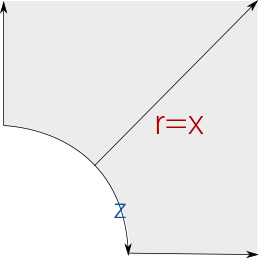
\includegraphics[width=60mm]{drawing102.png}
\end{center}
\begin{align}
\int x^s (C_s\circ B)|_{\Delta_b}=\frac{1}{s}\int_{\R}\Tr(\widehat{C_{s}\circ B}(\tau))d\tau+{}^{b}\Tr(A)+O(s)
\end{align}
where the second two terms goes to $0$ when $s=0$. Therefore for $\Re s>0$ and small, take into consideration of (294) we have
\begin{align}
\int [x_{s},A]B|_{\Delta_b}=\int_{\R}\Tr(\widehat{C}_{s}(\tau)\circ \widehat{B}(\tau))d\tau+O(s)
\end{align}
Now since $C_0=zA$, $\widehat{C_0}(\tau)=\widehat{zA}(\tau)$. We now calculate that 
\begin{align}
\widehat{zA(\tau)}&=-\frac{1}{i}\int \partial_{\tau}e^{-iz\cdot \tau}A|_{ff}(z)dz\\
&=\frac{-1}{i}\partial_{\tau}\int e^{-iz\cdot \tau}A|_{ff}(z)dz\\
&=-\frac{1}{i}\partial_{\tau}\widehat{A}_{\tau}
\end{align} 
Therefore we conclude that
\begin{align}
\int [x^{s} A]B|_{\Delta_b}=i\int_{\R}\Tr(\partial_{\tau}\widehat{A}(\tau))\widehat{B}(\tau)d\tau
\end{align}
and in our case $C_{s}\circ B$ is a holomorphic family of operators, which we discussed at Lecture 15. Recall that we have $C_{s}=z+sg(s,z)A=zA\in \Psi^{m,\alpha}_{b}(X)$. We note that the term $sg(s,z)A$ is bounded for $s\rightarrow 0$, and we can ignore. 
\remark 
Is the justification correct?
\exercise
Show that for $\Re s>0$ small, we have $sg(s,z)A\in \Psi^{m,\alpha}_b(X)$ is a holomorphic family. For $\delta$ chosen such that $|s|<\frac{\delta}{2}$, we have $|sg(s,z)|\le e^{\frac{\delta}{2}|z|}*C$. In particular we have
\begin{align}
g(s,z)=\frac{1}{2}z^2-\sum^{\infty}_{n=0}\frac{(-sz)^{n}}{(n+2)!}
\end{align}
and trivially we have 
\begin{align}
|sg(s,z)|\le s|z|^2 e^{|s||z|}\le s|z|^{2}e^{\frac{\delta}{4}|z|}\le Cs e^{\frac{\delta}{4}|z|}\le C' e^{\frac{\delta}{2}|z|}
\end{align}
So we are done with the ${}^{b}$-trace!
\begin{center}
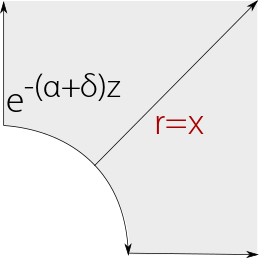
\includegraphics[width=60mm]{drawing103.png}
\end{center}
\remark
It seems missing a $1/2$ term in the expression for $g(s,z)$, and another $s$ term missing later. 
\subsection{Product structures}
\definition 
Consider $M_c=(-\infty, c]_{s}\times Y$. Let $E_0\rightarrow Y$ be a $\Z_2$-graded vector bundle. We can define $E\rightarrow M_c$ by $E_{(s,y)}=(E_0)_y$. In other words, where $\pi:(-\infty,0]_{s}\times Y\rightarrow Y: (s,y)\rightarrow y$. And $E$ is said to be of product type. Now let $g_0$ to be Rieamann metric on $Y$ such that $g=ds^{2}+g_0$ is the metric on $M_c$. Then $g$ is said of be of $\textbf{product type}$. 
\subsection{Clifford Action}
Now for all $p\in M_c$, we have $T_p^* M_c=\C\oplus T^{*}Y$. where $\R$ consists of the span of $ds$ factor, and $T_p^*$ is the domain for Clifford action. 

Let $\sigma$ be a linear map:
\begin{align}
\C\oplus \C T^{*}Y\rightarrow Hom(E_0)
\end{align}
such that $\sigma(\xi)^{2}=|\xi|^{2}$. here we may assume $\xi=\xi_1\cdot e_1+\eta, |e_1|=1, e_1\in \C$. Therefore $|\xi|^{2}=\xi_1^{2}+|\eta|^{2}$.

We require that $\sigma_0$ is odd with respect to the grading of $E_0$:
\begin{align}
\sigma_0(\xi):E^\pm_0\rightarrow E^\mp_0
\end{align}

Now from $\sigma_0$ we can define the Clifford action on the whole space as
\begin{align}
\sigma:\C T^*M_{c}=\C\oplus T^*Y\rightarrow Hom(E)
\end{align}
We know that $\xi=\xi_1ds+\eta$, therefore if for all $v\in E_{(s,y)}=E_{0}(y)$ we have 
\begin{align}
\sigma(\xi)(v)=\sigma_0(\xi_1 e_1+\eta)v
\end{align}
\remark
I am really confused with what (307) means and why it satisfies the required relationship. Did Prof.Loya meant to choose a random unit vector from $T^{*}Y$ and times $\xi_1$ to add it up to $\eta$?
\discussion 
On the other hand we can choose to working backwards to $\sigma_0$. Let \begin{align}
\nabla_0:C^{\infty}(Y,E_0)\rightarrow C^{\infty}(Y, T^{*}Y\times E_0)
\end{align} be a connection. Assume it is $\Z_2$ graded, Hermitian and Clifford action with respect to this action. Now for $\nabla_0$ we can define a new connection on $E$ as 
\begin{align}
\nabla=ds\otimes \partial s+\nabla_0, \nabla:C^{\infty}(M_C, E_{0})\rightarrow C^{\infty}(M_c, \C T^*M_c\oplus E_0), E_0=T^{*}Y
\end{align}
In this case we say that $\nabla$ is a connection of $\textbf{product type}$. 

\remark
It is still not clear to me how this relates to the discussion we had above. 

\exercise 
Let $\nabla$ to be $\Z_2$-graded, Hermitian, and compatible with the Clifford action. You do need to think what is the Levi-Civita connection of the product type manifold. I claim that we have
\begin{align}
\nabla^{LC}=\partial_{s}^{LC}+\nabla_{Y}^{LC}
\end{align}
this would involve Riemann metric, bundle, etc as well as product type $G$-structure. 
\remark 
Kind of unclear....
\subsection{Dirac operator}
If we have on $M_c$ a Riemannian metric, vector bundle $E$, Clifford actions, etc, which are all of product type, then we can define
\definition
\begin{align}
\eth=\frac{1}{i}\sigma\circ \nabla: C^{\infty}(M_c, E)\rightarrow C^\infty(M_c, E)
\end{align}
This operator is called $\textbf{product type}$ Dirac operator, also called the $\textbf{genuine Dirac operator}$, which is different from the $\textbf{generalized Dirac operator}$ that we are going to define later. 

\lemma
We have 
\begin{align}
\eth=\frac{1}{i}\sigma(ds)(\partial_{s}+D_0)
\end{align}
where $D_{0}:C^{\infty}(Y,E_0)\rightarrow C^{\infty}(Y, E_0)$. We claim that $\eth$ satisfies the following properties:
+
Self-adjointness:
\begin{align}
\langle \eth v, w\rangle=\langle v,\eth w\rangle
\end{align}
+
Anti-commutativity:
\begin{align}
-\sigma(ds)D_0=D_0 \sigma(ds)
\end{align}
+
$D_0$ is the even part of the $\Z_2$-grading of $E_0$. 
\proof
To prove it we write out $\eth$ explicitly:
\begin{align}
\eth&=\frac{1}{i}\sigma\circ \nabla\\
&=\frac{1}{i}\sigma(ds\otimes \partial_{s}+\nabla_0)\\
&=\frac{1}{i}\sigma(ds)\partial_{s}+\frac{1}{i}\sigma\circ \nabla_0\\
&=\frac{1}{i}(\sigma)(ds)(\partial_s+(ds)^{-1}\nabla_0)
\end{align}
We note that $D_0=(\sigma(ds)^{-1})(\sigma_0+\nabla_0)$ is even! 
\remark
unclear about where is this coming from. Is this about the second term $\frac{1}{i}\sigma\circ \nabla_0$? I think the term $\sigma(ds)\partial_{s}$ should be self-adjoint, but do not know a proof. 
\discussion
Recall that via (309) we have
\begin{align}
\nabla=ds\otimes \partial s+\nabla_0, \nabla:C^{\infty}(M_C, E_{0})\rightarrow C^{\infty}(M_c, \C T^*M_c\oplus E_0), E_0=T^{*}Y
\end{align}
and $\sigma_0\circ \nabla_0=\sigma_Y\circ \nabla_{0}$, with $\sigma_Y=\sigma_0|_{T^{*}Y}$. Therefore $\frac{1}{i}\sigma_{Y}\circ \nabla_0$ is a Dirac operator on $E_0\rightarrow Y$. Hence we have 
\begin{align}
D_0&=i\sigma(ds)^{-1}\frac{1}{i}\sigma_{y}\circ \nabla_0\\
&\rightarrow D_0^{*}=\frac{1}{i}\sigma_{y}\circ \nabla_0\circ (-i\sigma(ds))\\
&=-\sigma_{y}\circ \nabla_0\circ \sigma(ds)\\
&=-\sigma_{y}\circ \sigma(ds)\nabla_0\\
&=\sigma(ds)\sigma_{y}\circ \nabla_{0}\\
&=D_0
\end{align}
and we also have
\begin{align}
\nabla_{0}(\sigma(ds)v)&=\sigma(\nabla^{LC}ds)v+\sigma(ds)\nabla_0(v)\\
&=\sigma(ds)\nabla_0(v)
\end{align}
because we have $\nabla^{LC}(1 ds)=(\partial_{s}1)ds=0\cdot ds=0$. And the fact that $\sigma(ds)D_0=D_0\sigma(ds)$ can now be derived from self-adjointness. 
\remark
There seems to be some typos in the notes. Some of the derivations are unreadable to me. 

\discussion
We now have the following definition:
\definition 
Let $M$ be a manifold with a cylinderal end:
\begin{center}
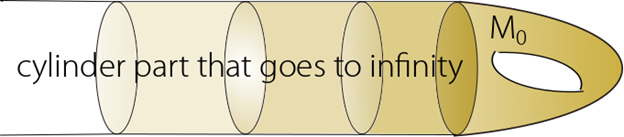
\includegraphics[width=100mm]{drawing38.png}
\end{center}
Let $g$ be a metric on $M$, let $E\rightarrow M$ be a $\Z_2$ graded Hermitian Clifford vector bundle. Let $\nabla$ be a $\Z_2$-graded Hermitian connection. Assume everything is product type as defined above on $M_c$, we call $D=\frac{1}{i}\circ \nabla$ a Dirac operator that is of product type on $M_c$. 

The following theorem earlier is concerning  $\eth=\frac{1}{i}\sigma(ds)(\partial_s+D_0)$ with $D_0:C^{\infty}(Y,E_0)\rightarrow C^{\infty}(Y,E_0)$ over $M_c$. We have:

\theorem 
If $D_0$ is invertible, then for all $\beta\in \R$ sufficiently small in absolute value, on appropriate domain we would have
\begin{align}
\textrm{Index} D=AS-\frac{1}{2}\eta
\end{align}
where $\eta$-invariant is given by
\begin{align}
\eta=\frac{1}{\sqrt{\pi}}\int^{\infty}_0 t^{-1/2}\Tr(D_0 e^{-tD_0^2})dt
\end{align}
\subsection{The $b$-category case}
We can extend this in the $b$-case. Let $x=e^s$, then we have 
\begin{align}
ds^{2}+g_0\rightarrow (\frac{dx}{x})^{2}+g_0
\end{align}
where as
\begin{align}
\nabla&\rightarrow ds\otimes \partial_{s}+\nabla_0\\
&=(\frac{dx}{x})\otimes x\partial_x+\nabla_0
\end{align}
In this case we call $\nabla:C^{\infty}(M,E)\rightarrow C^{\infty}(M, \C {}^{b}T^{*}X\otimes E)$ as a $b$-connection. We recall that we worked with $b$-differential operators earlier. 

Now in the interior we have $\eth=\frac{1}{i}\sigma(\frac{dx}{x})$, with $\sigma:\C T^{*}M\rightarrow Hom(E)$ be the Clifford action on $b$-cotangent bundle. On the boundary cylinder we have
\begin{align}
\eth=\frac{1}{i}\sigma(\frac{dx}{x})(x\partial_{x}+D_0)
\end{align}
and we have the index theorem in the $b$-category:

\theorem 
If $D_0^{-1}$ exists, then for $\beta\in \R$ that is sufficiently small, we have
\begin{align}
D^{+}:x^{\beta}\mathcal{S}^{0}(X,E^{+})\rightarrow x^{\beta}\mathcal{S}^{0}(X,E^{-})
\end{align}
is Fredholm. We also have $\textrm{Ind} D^{+}=\int_{X}AS+\frac{1}{2}\eta$, where $\eta$ is given by (329). 

\discussion 
Here we wish to discuss the ideas to construct the heat kernel. We want to work with generalized $b$-Laplacians. 
\example
Observe that over the collar of $X$, we should have $\eth^2=-(x\partial_x)^2+D_0^2$, with $\sigma(D_0^2)=g_0=|\eta|^{2}$, for all $\eta\in T^{*}Y$. So we define: 
\begin{center}
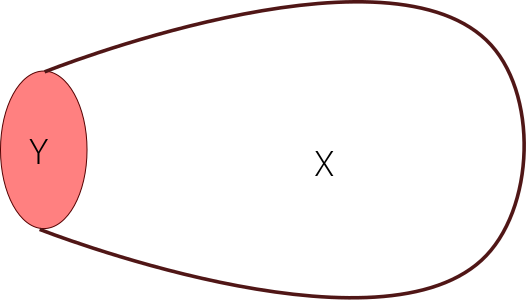
\includegraphics[width=60mm]{drawing83.png}
\end{center}

\definition 
A generalized $b$-Laplacian on $X$ is an operator $\Delta\in \textrm{Diff}^{2}_b(X,E)$ with $\sigma_{2}(\Delta)(\xi)=|\xi|^{2}$, for all $\xi\in {}^{b}T^{*}X$. It is of $\textbf{product type}$ on the collar if 
\begin{align}
\Delta=-(x\partial_x)^{2}+\Delta_0, \Delta_0\in \textrm{Diff}(X,E)
\end{align}
where $\Delta_0$ is a generalized Laplacian on the interior of $X$. 

\section{Lecture 19: Revisit the heat kernel for manifold with boundary}
\subsection{The gluing construction}
This will be the most difficult part of the proof of APS theorem, namely constructing the heat kernel. To review the set up, let $X$ be a generalized Laplacian. We ignore $E$ and we let
\begin{align}
\Delta:C^{\infty}(X)\rightarrow C^{\infty}(X), \Delta=-(x\partial_x)^{2}+\Delta_0
\end{align}
such that $(\sigma(\Delta)|\xi|)^{2}=|\xi|^{2}$. We recall the set up:
\begin{center}
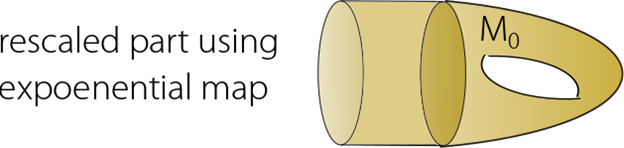
\includegraphics[width=100mm]{drawing39.png}
\end{center}
Our goal would be to construct the heat kernel for $\Delta$ operator. We want to construct \begin{align}
e^{-t\Delta}:S_{\beta}(X)\rightarrow S_{\beta}([0,\infty)\times X]
\end{align}
where $S_{\beta}(X)=x^{\beta}\mathcal{S}^{0}(X)$.
Here we want to be very precise: If $u\in S_{\beta}([0,\infty)\times X)$, then this is the same as $u(t,x)=x^{\beta}v(t,x)$. And if $v\in C^{\infty}([0,\infty)\times X)$ such that for all $k$ and $P\in \textrm{Diff}^{*}_b(X)$, we have $\partial^{k}_t P(v)\in L^{\infty}([0,\infty)\times X)$. In other words, $v$ has to be differentiable down to $0$. We want to construct solutions of $(\partial_t+\Delta)e^{-t\Delta}=0, e^{-t\Delta}|_{Id}$. 

To actually construct it we use a ``gluing'' idea coming from Melrose. It is really easy. We consider two functions $\phi, \psi_0\in C^{\infty}_{c}([0,\infty))$ such that
\begin{align}
\forall x\in [0,\frac{1}{2}], \phi(x)\equiv 1; \forall x\in [\frac{3}{4},\infty), \phi(x)\equiv 0; \phi\ge 0
\end{align}
\begin{center}
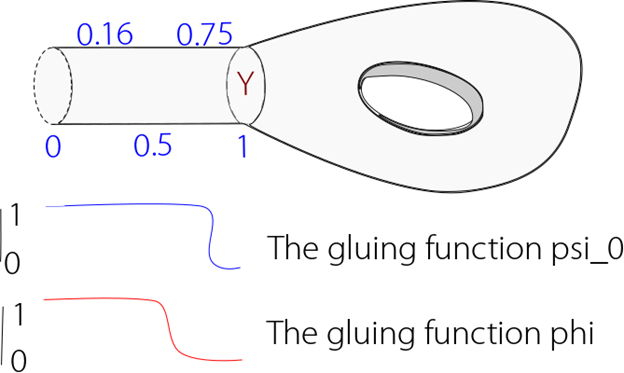
\includegraphics[width=120mm]{drawing105.png}
\end{center}
as well as
\begin{align}
\forall x\in [0,\frac{3}{4}], \psi_0(x)\equiv 1; \forall x\in [\frac{5}{6},1], \psi_0(x)\equiv 0; \forall x\in \textrm{supp}(\phi),\psi_0(x)\equiv 1
\end{align}
See the photo for the detail. We then choose $\psi_1\in C^{\infty}[0,\infty)$ such that $\psi_1\equiv 1$ on $[\frac{1}{2},\infty), \psi_1\equiv 0$ on $[0,\frac{1}{4}]$. Here is the essential idea by Melrose: 
\remark
For unknown reason $\phi,\psi_0$'s domains are different. Not sure why. 

\discussion 
To construct $e^{-t\Delta}$, we take heat kernel on $[0,1)\times Y$, and heat kernel on $X/[0,\frac{1}{2}]\times Y$. Then we glue them together. The heat kernel on $[0,1)\times Y$ can be taken to be
\begin{align}
H_{0}&=\frac{1}{\sqrt{4\pi t}}e^{-\frac{|z|^{2}}{4t}}e^{-t\Delta_0}, z=\log(\frac{x}{x'})\\
&=\frac{1}{\sqrt{4\pi t}}e^{-\frac{(\log(x)-\log(x'))^{2}}{4t}}e^{-t\Delta_0}
\end{align}
To see why, consider the operator
\begin{align}
\Delta:C^{\infty}(X)\rightarrow C^{\infty}(X), \Delta=-(x\partial_x)^{2}+\Delta_0
\end{align}
restricted to the collar $[0,1)_{x}\times Y$, which comes from the Laplacian from the cylinder: 
\begin{align}
\Delta:C^{\infty}(X)\rightarrow C^{\infty}(X), \Delta=-(\partial_r)^{2}+\Delta_0, x=e^{r}, r\in (-\infty, 0)
\end{align}
We can consider this on $(-\infty, \infty)_{r}\times Y$ instead. 
\remark
Can we really do that???
\discussion 
Now the heat kernel of $(-\partial_r)^{2}+\Delta$ is given by
\begin{align}
H_0=\frac{1}{\sqrt{4\pi t}}e^{-\frac{(r-r')^{2}}{4t}}e^{-t\Delta_0}
\end{align}
We transform back to the collar by $x=e^{r}, x'=e^{r'}$ and we get equation (348). 

It is clear that for $t>0$, as $z\rightarrow \infty$, we have $H_0(z)$ in (347) decreases faster than any exponential power. Therefore the heat kernel is in the $\textbf{small calculus}$ defined in Lecture 11. 

Now using the cut-off function $\phi, \psi_0$ we have
\begin{align}
\psi_0 H_0 \phi&=\psi_0(x)\phi(x')\frac{1}{\sqrt{4\pi t}}e^{-\frac{|z|^{2}}{4t}}e^{-t\Delta_0}\in \Psi^{-\infty}_{b}(X), \forall t>0
\end{align}
They are in $\Psi^{-\infty}_b(X)$ because after introducing the cut-off, $\psi_0 H_0\phi$ has kernel supported in the following region in $X^2_b$:
\begin{center}
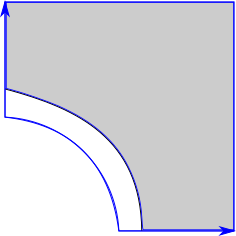
\includegraphics[width=60mm]{drawing106.png}
\end{center}
Let us check explicitly:

\lemma
We claim that
\begin{align}
\forall \beta>0, \psi_0 H_0 \phi: S_\beta (X)\rightarrow S_\beta([0,\infty)\times X)
\end{align}
as well as
\begin{align}
\psi_0 H_0 \phi|_{t=0}=\phi\cdot Id
\end{align}
\proof
Prof. Loya initially wanted to leave this as an exercise, but decided to do it in the lecture. 

The idea is very nice. We let $\mu(x)\in S_\beta(X)=x^{\beta}S{0}(X)$.  Now write out explicitly we have 
\begin{align}
\psi_0 H_0 \phi \mu(x)=\frac{1}{\sqrt{4\pi t}}\int \psi_0(x)e^{-\frac{(\log(x)-\log(x'))^{2}}{4t}}e^{-t\Delta_0}\phi \mu(x',y)\frac{dx'}{x'}
\end{align}
We now make the change of variable:
\begin{align}
\omega=\frac{\log(x)-\log(x')}{2\sqrt{t}}
\end{align}
Then we have
\begin{align}
e^{2\sqrt{t}\omega}&=e^{\log(x)-\log(x')}\\
&=\frac{x}{x'}\\
&\rightarrow x'=xe^{-2\sqrt{t}\omega}
\end{align}
Therefore we can change the density factor by
\begin{align}
\frac{dx'}{x'}&=\frac{x(-2\sqrt{t})e^{-2\sqrt{t}\omega}d\omega}{xe^{-2\sqrt{t}\omega}}\\
&=-2\sqrt{t}d\omega
\end{align}
Substitute this into (355) and make the change of variable $t=s^{2}$, we have
\begin{align}
(\phi_0 H\phi)\mu&=\frac{1}{\sqrt{4\pi t}}\int \psi_0 e^{-\omega^{2}}e^{-t\Delta_0}(\phi \mu)(xe^{-2\sqrt{t}\omega}, y)d\omega (2\sqrt{t})\\
 &=(\psi_0 H_0 \phi u)|_{t=0}\frac{1}{\sqrt{\pi}}\int e^{-\omega^2}(\phi \mu)(x)d\omega\\
 &=\frac{1}{\sqrt{\pi}}\int_{\R}e^{-\omega^{2}}(\phi \mu)(x)d\omega\\
 &=\psi_0(x)\phi(x)\mu(x)
\end{align}
where we used the fact that odd power goes away after we replace $t=s^{2}$. 
\qed
\remark
I really do not understand how Prof. Loya went from the second line to the third line. Did we just take $t=0$ and pull everything out? But this seems only verified the second claim of this lemma. I also do not see how the "odd power" thing is useful anywhere. 
\discussion
Here is a little remark by Prof. Loya:
\exercise
Show that $\psi_0H\phi(\mu)\in S_{\beta}([0,\infty)\times X)$.
\discussion 
This is from last year's lecture on Atiyah-Singer index theorem. We know that there exist $H_1\in \Psi^{-2}(X)$, with $X'=X/([0,\frac{1}{4})\times Y)$ such that
\begin{align}
(\partial_t+\Delta)H_1=R_1
\end{align}
where $R=R(t,x,x')$ and $R\in C^{\infty}([0,\infty)\times X'\times X')$. We also require that $R\equiv 0$ at $t=0$, which implies $\partial^{k}R|_{t=0}=0,\forall k\in \N$.  This is possible because in this case $X'$ is $\textbf{manifold without boundary}$. See the following graph:
\begin{center}
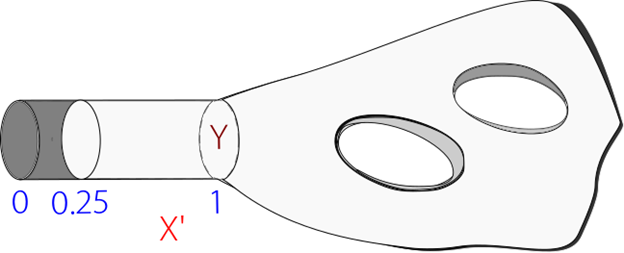
\includegraphics[width=100mm]{drawing108.png}
\end{center}
\remark
There seems to be some confusion with $R_1$ and $R$ in the notes, as well as whether we should use $R(t,x,x)$ or $R(t,x',x')$, etc. It seems likely to confuse the reader to think $x\in X, x'\in X'$, etc, though this is clear from the context. 
\discussion
Recall, we can patch $X'$ by finitely many coordinate patches, each of which is differeomorphic to $\R^{n}$. On each coordinate patch, we can find a $Q$ that satisfies our iterative equation $*$. Then we just need a partition of unity argument to finish the task!

\remark
Unclear what "$*$" refers to. What does $Q$ really mean at here? The same as used in later context? 

\discussion
We now try to consider the cut-off heat kernel $\phi_1 H_1 (1-\phi)$. We have the following graph:
\begin{center}
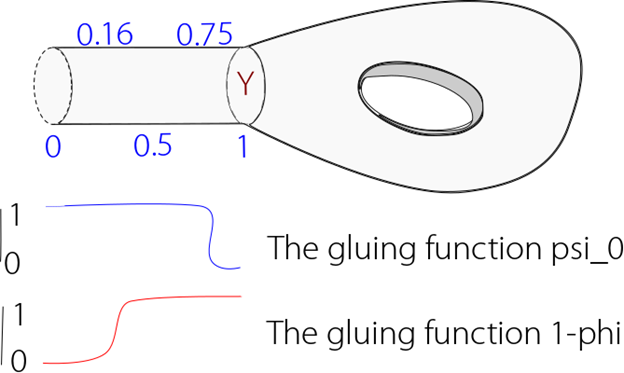
\includegraphics[width=100mm]{drawing109.png}
\end{center}
\remark 
With all respect, in retrospect I feel we did not even define $\psi_1$. 

\discussion
And we can visualize the support of its Schwartz kernel from the following graph:
\begin{center}
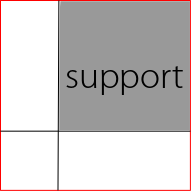
\includegraphics[width=60mm]{drawing110.png}
\end{center}
Now it is $\textbf{easy}$   to check that for $t>0$, the kernel $\psi_1 H_1 (1-\phi)\in \Psi^{-\infty}$ is  $C^{\infty}$ in $X^2$ vanishing near the boundary of $X^2$.
\remark
Is this because its support is off the front face? 
\discussion 
In particular we have
\begin{align}
\Psi_1 H_1 (1-\phi):S_\beta (X)\rightarrow S_{\beta}([0,\infty)\times X)
\end{align}
as well as
\begin{align}
\Psi_1 H_1 (1-\phi)|_{t=0}=\Psi_1 (1-\phi)|_{Id}=(1-\phi)\cdot Id
\end{align}
\subsection{The patched up heat kernel}
Now we can define the heat kernel over the whole manifold: 
\begin{align}
Q=\Psi_0H_0\phi+\Psi_1H_1(1-\phi)
\end{align}
Then we have:
\begin{align}
Q:S_{\beta}(X)\rightarrow S_{\beta}([0,\infty)\times X)
\end{align}
as well as
\begin{align}
Q|_{t=0}&=\phi\circ Id+(1-\phi)\circ Id\\
&=Id
\end{align}
and because the sum of operators in $\Psi^{-\infty}_b(X)\in \Psi^{-\infty}_b(X)$, we have $Q\in \Psi^{-\infty}_b(X)$. Finally we have the expected theorem:

\theorem 
We have $(\partial_t+\Delta)Q=R$, where $R\in C^{\infty}([0,\infty)\times X\times X)$ and $R\equiv 0$ at $t=0$ and at the boundary $\partial X^2$. 

\proof
To prove it, we use the well known $\textit{Duhamel's formula}$:
By definition we have
\begin{align}
(\partial_t+\Delta)Q&=(\partial_t+\Delta)(\Psi_0H_0\phi+\Psi_1H_1(1-\phi))
\end{align}
Expand out the first term using Leibniz's rule we have
\begin{align}
(\partial_t+\Delta)\Psi_0(x)H_0\phi&=(\partial_t-(x\partial_x)^{2}+\Delta_0)\Psi_0H_0\phi\\
&=\Psi_0(\partial_t-(x\partial_x)^{2}+\Delta_0)H_0\phi-(x\partial_x)^{2}\Psi_0 H_0 \phi-2(x\partial_x \Psi_0)(x\partial_x H_0)\phi\\
&=-(x\partial_x)^{2}\Psi_0H_0 \phi-2(x\partial_x \Psi_0)(x\partial_x H_0)\phi\\
&=R_0
\end{align}
where the first term vanishes because $H_0$ is the heat kernel. 
\remark
I asked in class why there is no third term involved like $(x\partial_x)^{2}\phi$, is this because writing out the kernel we only have $\phi(x')$ part?. Do not remember Prof. Loya's answer on this.  
\discussion
Now we can look at the kernel of $R_0$: We claim it is in the following region:
\begin{center}
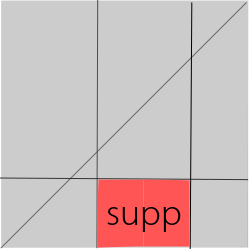
\includegraphics[width=60mm]{drawing111.png}
\end{center}
This is because $D\Psi_0$ vanishes when $\Psi_0\equiv 1$ in the region $[0,\frac{3}{4}]$. In particular the region is $\textbf{below}$ the diagonal.  Therefore it should be zero near a neighborhood of the diagonal. 
\remark
Still unclear why it must be below the diagonal. There should be a small box on the diagonal where it is not zero by the above argument. Even more puzzling is why the support is in one region, but not two regions if the diagonal has to be escaped. 
\discussion 
We can now write it out explicitly:
\begin{align}
R_0\in C^{\infty}([0,\infty)\times X^2)
\end{align}
and $R_0\equiv 0$ at all boundary points. We now take the first operator from (376) and try to reorganized it:
\begin{align}
T=\Psi(x)\frac{(x\partial_x)^{2}\Psi_0}{\sqrt{4\pi t}}e^{-\frac{|z|^{2}}{4t}}e^{-t\Delta_0}\phi(x')
\end{align}
Now given $u$ we have
\begin{align}
Tu=\frac{1}{\sqrt{4\pi t}}\int \Psi(x)\frac{(x\partial_x)^{2}\Psi_0}{\sqrt{4\pi t}}e^{-\frac{|z|^{2}}{4t}}e^{-t\Delta_0}\phi(x')\mu(x')\frac{dx'}{x'}
\end{align}
where the part corresponding to the $e^{-t\Delta_0}\rightarrow 0$ when $z=0$ at the diagonal. 
\remark
Not very clear to me why this is true. 
\discussion
We have the following lemma:
\lemma
If $\Psi(x,x')\in C^{\infty}_{c}([0,1)\times [0,1))$, $\Psi\equiv 0$ for $|x-x'|<\delta$, $\delta>0$, then we have
\begin{align}
\frac{\Psi}{\sqrt{4\pi t}}e^{-|z|^{2}}e^{-t\Delta_0}\in C^{\infty}([0,\infty)_{t}\times X^2)
\end{align}
and it is $0$ at all boundary points. 
\proof
Unfortunately Prof. Loya got stuck with the proof. He claim that the first step is to let $|z|<\delta_1$, then divide the whole expression by $z$, and so on. Adam suggested that there may be some better approach, Prof. Loya claimed that the second claim should be true heuristically since at $|z|=\infty$ the above expression vanishes, and the first claim somehow also magically follows as everything is in small calculus. I am totally lost. 
\discussion
The second part of (373) can also be expanded out explicitly and computed. After some computation we have
\begin{align}
(\partial_t+\Delta)\Psi_1 H_1 (1-\phi)&=\Psi(\partial_t+\Delta)H_1(1-\phi)-(x\partial_x)^{2}\Psi_1 H_1 (1-\phi)-2(x\partial_x)\Psi_1(x\partial_x H_1)(1-\phi)\\
&=R_1
\end{align}
And a similar Lemma like Lemma 7 would hold in our case via similar logic. In conclusion we have $\mu(t,x,x')\in C^{\infty}([0,\infty)_{t}\times [0,1)\times [0,1))$, as well as $\partial^k_{t} \partial^{l}_{x} \partial^{m}_{x'} \equiv 0$, whenever $t,x,x-x'\rightarrow 0$. Using ``similar logic'' we have $R_1\in C^{\infty}([0,\infty)\times X\times X)$, and $R_1\equiv 0$ at all the boundary points. 
\qed
\remark
Needless to comment, I believe this ``proof'' needs serious polishing. Otherwise I think only Adam can follow it. 
\discussion
Now we just need to get rid of $R$. Recall that we have 
\begin{align}
(\partial_t+\Delta)Q=R, Q|_{t=0}=Id
\end{align}
as well as
\begin{align}
R\in C^{\infty}([0,\infty)\times X^2)), R_{\partial X^2}=0
\end{align}
To get rid of $R$ we use the Duhamel's principle. There should exist $H$ such that $(\partial_t+\Delta)H=0$, and $H|_{t=0}=Id$ as well as $G$ such that $(\partial_{t}+\Delta)G=Id$, and $G|_{t=0}=0$. We can write out $H,G$'s relationship precisely as
\begin{align}
G\mu(t)=\int^{t}_{0}H(t-s)\mu ds, H=\partial_t G
\end{align}
and we would need to construct $G$ in order to construct $H$. 
\subsection{Step 1}
Consider $\mathcal{H}_{\beta}$ for the heat space which consists of functions $\mu(t,x)=x^{\beta}v(t,x), v\in C^{\infty}([0,\infty)\times X)$ such that $\partial_{t}^{k}Pv\in L^{\infty}, \forall k, \forall P\in \textrm{Diff}^{*}_b$. \\
Now define
\definition
$G_{Q}:\mathcal{H}_{\beta}([0,\infty)\times X)\rightarrow \mathcal{H}_{\beta}([0,\infty)\times X)$ is defined by
\begin{align}
Gu=\int^t_0 Q(t-s)\mu(s)ds
\end{align}
Observe for all $\mu\in S_{\beta}(X)$ we now have 
\begin{align}
(\partial_{t}+\Delta_0)C_{Q}\mu=(I+C_{R})\mu(s), C_{R}\mu=\int^{t}_{0}R(t-s)\mu(s)ds
\end{align}
This can be verified formally:
\begin{align}
(\partial_t+\Delta_0)(\int^{t}_0 Q(t-s)\mu(s)ds)&=\mu(t)+\int^{t}_{0}(\partial_t+\Delta)Q(t-s)\mu(s)ds\\
&=(I+C_R)\mu
\end{align}
The idea is now somehow to invert $C_R$ so that we have $(\partial_t+\Delta)G=Id$. We now fix any $\epsilon>0, t_0>0$, and consider the vector space
\begin{align}
V=x^{\epsilon}x'^{\epsilon}C^{0}([0,t_0]\times X\times X)
\end{align}
with the norm $\mu=x^{\epsilon}x'^{\epsilon}$, $|\mu|=|v|_{\infty}$. Then the vector space $V$ is complete. Now let $f,g\in V$, we define their convolution to be
\begin{align}
(f*g)(s)(x,x')=\int \int f(t-s, x, \omega)g(s,\omega, x')\frac{d\omega}{\omega}
\end{align}
where $\frac{d\omega}{\omega}$ is the $b$-density on $X$. 
Here is the idea to invert. To invert
\begin{align}
(\partial_{t}+\Delta_0)C_{Q}=(I+C_{R})
\end{align}
We use the familiar Newmann series:
\begin{align}
I+\sum^{\infty}_{i=1}(-1)^{i}C^{i}_R
\end{align}
where the power is the composition. We have the following lemma to characterize the Newmann series:
\lemma
\begin{align}
C_R\circ C_R=C_{R\times R}, (C_{R})^{k}=C_{R\cdots R}
\end{align}
\proof
In order to prove this lemma, we need to prove the following lemma:
\lemma
For all $f,g\in V$, we have
\begin{align}
|f*g|\le C_0 |f| |g|, C_0=\int_{X}x^{2\epsilon}\frac{dx}{x}
\end{align}
\proof
We have
\begin{align}
f=x^{\epsilon}(x')^{\epsilon}\tilde{f}(t,x,x'), g=x^{\epsilon}x'^{\epsilon}\tilde{g}(t, x,x')
\end{align}
Therefore the convolution is given by
\begin{align}
(f*g)(t,x,x')&=\int_0^{t}\int_{X}x^{\epsilon}\omega^{\epsilon}\tilde{f}(t-s, x, \omega)\omega^{\epsilon}(x')^{\epsilon}\tilde{g}(t,\omega, x')\frac{d\omega}{\omega}\\
&=x^{\epsilon}(x')^{\epsilon}\int^t_0\int_{X}\omega^{2\epsilon}\tilde{f}(t-s, x,\omega)\tilde{g}(s,\omega, x')\frac{d\omega}{\omega}
\end{align}
This implies in particular that
\begin{align}
|f*g(t_0)|&\le \int^{t}_0C_0|f||g|\\
&=t_0c_0|f||g|\\
&\rightarrow |f*g|<c_0 |f||g|
\end{align}
This proved Lemma 9.\qed \\
Lemma 9 now implies the following theorem:
\theorem 
For all $f\in V, k\in \Z, k\ge 0$, we have
\begin{align}
|f^{k}|\le \frac{(C_0 t_0)^{k-1}}{(k-1)!}|f|^{k}
\end{align}
\remark
It is not clear why we have a $\frac{1}{(k-1)!}$ factor. Iterating Lemma 9 we would only have $|f^{k}(t)|\le (C_0 t_0)^{k-1}|f|^{k}$. I would have guessed the $\frac{1}{(k-1)!}$ factor coming from the simplicial decomposition of the space $[0,t]^{2}$, using description of a simplex being like $\{0\le s_1\le s_2\cdots \le t\}$. But this should be made very clear, otherwise it can be quite confusing. 
\discussion
We now let 
\begin{align}
S&=\sum^{\infty}_{k=1}(-R)^{k}\\
&=\sum^{\infty}_{k=1}(-R)*\cdots (-R), R\in V
\end{align}
and by Theorem 31 this sum converges in $V$. We claim $S\in C^{\infty}([0,t_0])\times X\times X)$. The argument is familiar: We use $S=-R+R\times R-R*S*R$ and write out the kernel explicitly to show it is infinitely differentiable. 
\remark
The notes says "$S\equiv 0$ in Taylor series". Not sure what that means. Does Prof. Loya meant $R+S+R*S$?
\discussion
We now consider $C_S$. We have
\begin{align}
(I+C_R)(I+C_S)&=I+C_R+C_S+C_R\circ C_S\\
&=I+C_{R+S+R*S}\\
&=I+C_0\\
&=I
\end{align}
This finished proof of Lemma 8
\qed 
To summarize we now have
\begin{align}
(\partial_t+\Delta)Q&=R\\
&\rightarrow (\partial_t+\Delta)C_{Q}=I+C_{R}\\
&\rightarrow (\partial_t+\Delta)C_{Q}(I+C_{S})=I\\
&\rightarrow (\partial_t+\Delta)(C_{Q}+C_{Q*S})=I\\
&\rightarrow (\partial_t+\Delta)G=I, G=C_Q+C_{Q*S}, G|_{t=0}=0\\
&\rightarrow H=\partial_{t}G
\end{align}
Therefore since we know $e^{-t\Delta_0}$ exists, $Q$ exists, and we have $H=\partial_{t}G=Q+Q*S$. As a result $e^{-t\Delta}$ also exists. 
\subsection{Step 2}
From above discussion we know $H=\Psi_1 H_0 \phi+\Psi_2 H_1(1-\phi)+Q*S$. Prof. Loya now give the following exercise:

\exercise
Using that $S\in C^{\infty}([0,\infty)\times X\times X)$ and $S\equiv 0$ in Taylor series at all boundary points to prove that $Q*S$ belongs to the same space. 

\proof
$Q*S$ exists and vanishes at the boundary is not difficult given the composition formula (392) regarding their kernels. However to show $Q*S\in C^{\infty}[0,\infty)\times X\times X$ requires much more work and we have to use (399) as theorems to differentiate under the integral sign, since relationship like  $S=-R+R\times R-R*S*R$ exists between $Q, R$. 
\qed\\
To summarize we now have the following theorem:
\theorem 
For all $t>0$, we have $e^{-t\Delta}\in \Psi^{-\infty}_b(X)$ . As $t\rightarrow 0$ we have
\begin{align}
e^{-t\Delta}|_{\Delta_b}\sim t^{-\frac{n}{2}}\sum^{\infty}_{k=0}a_kt^{k}, a_k\in C^{\infty}(X, \Omega_b)
\end{align}
\proof
We know that
\begin{align}
(Q*S)|_{\Delta_b}\equiv 0
\end{align}
because $Q*S\equiv 0$ at $t=0$ in Taylor series. 
\remark
This is not clear to me. We do know $G|_{t=0}=0$, but this is trivial. And we have not shown $Q*S|_{t=0}=0$, in fact we have no idea what $S$ is, and we know that $Q|_{t=0}=Id$, see(384). 
\discussion
We know that restricted over the $b$-diagonal we have
\begin{align}
\Psi_1 H_1 (1-\phi)|_{\Delta_b}=(1-\phi)H_1|_{\Delta}
\end{align}
because $(1-\phi)\equiv 0$ near the front face. 
\begin{center}
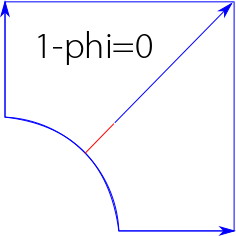
\includegraphics[width=60mm]{drawing112.png}
\end{center}
We have $H_1\in \Psi^{-2}_{H}(X'), H_1|_{\Delta}\sim t^{-\frac{n}{2}}\sum^{\infty}_{k=0}a_k'$, where $a_k'\in C^{\infty}_{c}(X, \Omega_b)$. 
\remark
I am a bit confused. Does Prof. Loya meant $\Psi_1\equiv 1$ near the front face, and $(1-\phi)\equiv 0$ near the front face?
\discussion 
Finally we have the net formula to be
\begin{align}
(\Psi_0 H_0 \phi)|_{\Delta_b}&=\frac{\Psi_0(x)}{\sqrt{4\pi t}}e^{-\frac{|z|^{2}}{4t}}e^{-t\Delta_0(y,y')}\phi(x')|_{\Delta_b}\\
&=\frac{\phi(x')}{\sqrt{4\pi t}}e^{-t\Delta_0}(y,y')\frac{dx'}{x'}, z=0, z\in \Delta_b
\end{align}
We know that the dimension of $Y$ is $n-1$. Therefore we have analogous heat kernel expansion like (416):
\begin{align}
e^{-t\Delta_0}(y,y)\sim t^{-\frac{n-1}{2}}t^{k}\sum a''_{k}(y)
\end{align}
In conclusion we have
\begin{align}
(\Psi_0 H_0 \phi)|_{\Delta_b}&=t^{-\frac{n}{2}}\sum^{\infty}_{k=1}\frac{\phi(x)}{\sqrt{4\pi}}a_k''(y)\frac{dx}{x}\in C^{\infty}(X, \Omega_b)
\end{align}
as well as 
\begin{align}
e^{-t\Delta}|_{\Delta_b}\sim t^{-\frac{n}{2}}\sum^{\infty}_{k=0}a_kt^{k}, a_k\in C^{\infty}(X, \Omega_b)
\end{align}
\remark
Are we in some essential sense done once we derived (422)? 

\subsection{Return to the Dirac case}
In practice, all applications of Atiyah-Singer theorem is based on Dirac operators. We assume that we have a Dirac operator $\eth: C^{\infty}(X, E)\rightarrow C^{\infty}(X,E)$ which is of product type Clifford operator. Therefore
\begin{align}
\eth^2=\frac{1}{i}\sigma\circ \nabla
\end{align}
where $\nabla$ is a $\Z_2$-graded Clifford connection. Since $\eth^2$ is a generalized Laplacian, we can consider the point-wise super-trace:
\begin{align}
str(e^{-t\eth^2}|_{\Delta_b})&=\Tr (e^{-t\eth^{-}\eth^{+}}|_{\Delta_b})-\Tr(e^{-t\eth^{+}\eth^{-}}|_{\Delta_b})
\end{align}
For all $p\in \Delta_b$, we know $e^{-t\eth^2}(p,p)\in Hom(E_p)=Hom(Z_p^+\oplus Z_p^-)$. We thus take super-trace on $E_p$ by expanding out the heat kernel. Observe that we have
\begin{align}
str(e^{-t\eth^{2}}|_{\Delta_b})\sim t^{-\frac{n}{2}}\sum^{\infty}_{k=0}t^{k}b_k, b_k\in C^{\infty}(X, \Omega_b)
\end{align}
We thus recover the local index theorem as we promised in Lecture 1, but this time we are fully rigorous:

\theorem 
If $X$ is even dimensional, then $str(e^{-\eth^{2}}|_{\Delta_b})\sim AS+O(t)$. 
\proof
Our time is almost up and let me sketch a proof really quick. From (426) we know that
\begin{align}
str(e^{-t\eth^{2}}|_{\Delta_b})\sim t^{-\frac{n}{2}}\sum^{\infty}_{k=0}t^{k}b_k, b_k\in C^{\infty}(X, \Omega_b)
\end{align}
We need to show that $b_k\equiv 0$ for $k<\frac{n}{2}$ for the interior of $X$ and $b_k$ are 

\remark
The notes on this is barely legible, needs some correction. 
\subsection{Homework for Lecture 19}

\section{Lecture 20: Proof of APS theorem}

\section{Lecture 21: In-depth study of the eta-invariant}

\section{Lecture 22:Semi-classical operators and blow up space}

\section{Lecture 23: Construction of heat kernel in semi-classical operators}

\section{Lecture 24: Symbol spaces of heat kernel in semi-classical operators}


\end{document}
